\documentclass[11pt]{article}
\usepackage[a4paper, hmargin={2.8cm, 2.8cm}, vmargin={2.5cm, 2.5cm}]{geometry}
\usepackage{eso-pic} % \AddToShipoutPicture
\usepackage{graphicx} % \includegraphics
\usepackage{amsmath}
\usepackage{tabto}
\usepackage[hidelinks]{hyperref}
\usepackage{enumerate}
\usepackage{txfonts}
\usepackage{graphicx}
\usepackage{float}
\usepackage{listings}
\usepackage[space]{grffile}
\usepackage{tabularx} % \For resizing tables
\usepackage{color, colortbl}
\usepackage{xcolor}
\lstset { %
    language=C++,
    backgroundcolor=\color{black!5}, % set backgroundcolor
    basicstyle=\footnotesize,% basic font setting
}
\hypersetup{breaklinks=true}

%% Change `ku-farve` to `nat-farve` to use SCIENCE's old colors or
%% `natbio-farve` to use SCIENCE's new colors and logo.
\def \ColourPDF {include/ku-farve}

%% Change `ku-en` to `nat-en` to use the `Faculty of Science` header
\def \TitlePDF   {include/nat-en}  % University of Copenhagen

\title{
  \vspace{3cm}
  \Huge{Bellman Ford, Dijkstra's, and A* search} \\
  \Large{Analysis and implementation of 3 shortest path algorithms}
}

\author{
  \Large{Iversen, Bjarke Kingo}
  \\ \texttt{bjarkekingo50@gmail.com} \\\\
  \Large{Truong, Susanne}
  \\ \texttt{suzze-t@hotmail.com}
}

\date{
    \today
}

\begin{document}

\AddToShipoutPicture*{\put(0,0){\includegraphics*[viewport=0 0 700 600]{\ColourPDF}}}
\AddToShipoutPicture*{\put(0,602){\includegraphics*[viewport=0 600 700 1600]{\ColourPDF}}}

\AddToShipoutPicture*{\put(0,0){\includegraphics*{\TitlePDF}}}

\clearpage\maketitle
\thispagestyle{empty}

\newpage

%% Write your dissertation here.
\section{Abstract}
In this thesis we present and discuss three shortest path algorithms; Bellman Ford, Dijkstra's algorithm, and A* search. We analyse the algorithms and their time complexities using the binary heap data structure. The algorithms are then implemented in C++ and undergo a benchmark test, where we measure the CPU time among other things. The benchmark showed that the difference in CPU time grew heavily when computing larger amounts of data, using the different algorithms. Bellman Ford performed the worst by a wide margin, while A* search performed the best.


\newpage
\tableofcontents
\newpage
%%%%%%%%%%%%%%%%%%%%%%%%%%%%% Introduction %%%%%%%%%%%%%%%%%%%%%%%%%%%%%
\section{Introduction}
It is widely known that it can be time-consuming to choose the wrong path, if you want to travel from one city to another. It will most certainly be faster to aboard the train from Chicago to Seattle, rather than going through Los Angeles before heading to Seattle. Choosing the shorter path may therefore save a lot of time. A shortest path can be seen as a path between two points where the total distance cannot be less than this, if we take another route. \\

\noindent The problem herein is that in lots of cases it is nowhere intuitive which path that guarantees the consumption of time to be minimal. We probably cannot withstand the big amounts of information if we should compute the shortest path, through millions of combinations by ourselves. For computersystems to choose such a path, they would need a method for calculating such. We call such a method an algorithm.\\

\noindent Different shortest-path algorithms are known to solve such problems theoretically. In this thesis, we will examine the theory behind these algorithms and prove their correctness. We will also analyse whether the time-complexity given by Bellman Ford and Dijkstra's algorithms holds in real life implementations, by implementing them with a binary heap in C++. Furthermore, we also analyse and implement the A* search algorithm to see how well Bellman Ford and Dijkstra's algorithm match up against this on Euclidean planar graphs.\\

\section{Problem definition}
To examine and benchmark the complexity of different shortest-path algorithms, e.g. Dijkstra's algorithm, Bellmann Ford, and A* search. We will do this by implementing and comparing them using different data structures and libraries. Finally we will compare the results of these experiments with the theoretical bounds.

%%%%%%%%%%%%%%%%%%%%%%%%%%%%%%% Notation %%%%%%%%%%%%%%%%%%%%%%%%%%%%%%%
\section{Notation}
A short list of notations used throughout the thesis:
\begin{itemize}
\item $G(V,E)$ = Graph, consisting of a set of vertices V, and a set of edges E.
\item $s$ = Designated to be the source vertex s.
\item $t$ = Designated to be the target vertex t.
\item $w(u,v)$ = Weighted distance from vertex u to v.
\item $d[v]$ = The weigth of the current shortest path from s to v. $d[s]$ is initialized to be 0.
\item $\pi[v]$ = Predecessor/parent vertex to v in the current shortest path. This is set to a vertex once/if a shorter path is discovered from s to v.
\item $\delta(u,v)$ = the weigth of the shortest path from u to v.
\item lg(n) = $log_{2}$(n).
\item $\{v_{1}, v_{2}, ..., v_{k}\}$ a path from some start-vertex containing k vertices in succeeding order.
\item $u \rightarrow v$ = a direct path from $u$ to $v$ connected by 1 edge.
\item $u \rightsquigarrow v$ = a path from $u$ to $v$ going through one or more vertices.
\item $h(v)$ = Heuristic function used on vertex v, for a more detailed description see section 10.2.
\end{itemize}

%%%%%%%%%%%%%%%%%%%%%%%%%%% Shortest Paths %%%%%%%%%%%%%%%%%%%%%%%%%%%
\section{On Shortest Paths}
In the shortest path problem, a graph $G = (V,E)$ is given, where $V$	
is the set of vertices, and $E$ is the set of edges. Each edge
connects two vertices and contains a weight, indicating the cost of
moving between these vertices. By using a shortest path algorithm, we
can find a shortest path $P = \{s, v_{1}, v_{2}, ..., v_{k}\} \in V$ from a
given source vertex $s \in V$ to all other vertices $v \in V$. I.e., for all vertices, we want to find a path, where the total weight of the visited edges is minimal.\\

\noindent We can compute the total sum of weights in a path P containing k vertices thus:\\
$$w(P) = \displaystyle\sum_{i=1}^{k} w(v_{i-1},v_i)$$

%%%%%%%%%%%%%%%%%%%%%%%%%%%%% Relaxation %%%%%%%%%%%%%%%%%%%%%%%%%%%%%
\noindent
\subsection{Initialization and relaxation}
When searching for the shortest path from a source vertex $s$ to a
vertex $v$, a shortest-path estimate $d[v]$ is preserved for each
vertex $v \in V$. To initialize the estimate and predecessor for all vertices, the following function is used:\\

\textbf{INITIALIZE-SINGLE-SOURCE$(G, s)$}
\begin{enumerate}
\NumTabs{24}
\setlength\itemsep{0em}
\item \textbf{for } each vertex $v \in G.V$
\item \tab{$d[v] = \infty$}
\item \tab{$\pi[v] = NIL$}
\item $d[s] = 0$
\end{enumerate}
The shortest-path estimate for the source is 0, since this is where the algorithm begins. The other vertices' distance is set to $\infty$, since the path from $s$ to a vertex $v$ is unknown at start. Not knowing the path also results in the predecessor being unknown, which is why $\pi[v]$ is set to NIL.\\
At first, $d[v]$ will be an overestimate, but if we see that the shortest path to $v$ can be improved by going through a vertex $u$, we update the estimate $d[v]$ with the new and lower cost. As better paths are found, we will eventually get the correct shortest-path estimate and find the shortest path, if it exists. This technique is called relaxation and is used by the three algorithms that we will talk about later. The pseudocode for relaxing an edge $(u,v) $ is shown below:\footnote{Introduction to Algorithms, pg. 649, CLRS}\\

\textbf{RELAX$(u, v, w)$}
\begin{enumerate}
\NumTabs{24}
\setlength\itemsep{0em}
\item \textbf{if } $d[v] > d[u] + w(u,v)$
\item \tab{$d[v] = d[u] + w(u,v)$}
\item \tab{$\pi[v] = u$}
\end{enumerate}
If the current distance from a source to the vertex $v$ is larger than the path going through vertex $u$ to $v$, the estimate is updated. The predecessor for $v$ will then be $u$. The next figure illustrates the procedure of relaxing an edge $(u,v)$.

\begin{figure}[H]
\centering
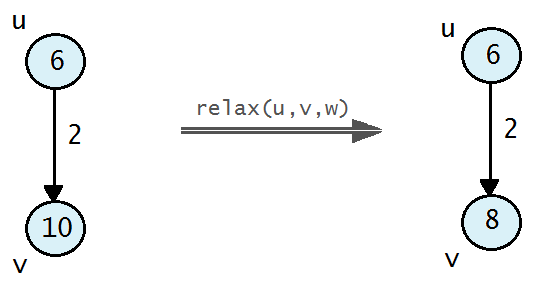
\includegraphics[scale=0.4]{Pictures/Relaxation-example.png}
\caption{Relaxing an edge $(u,v)$.}
\end{figure}

\noindent Before relaxing the edge, we have that $d[v] > d[u] + w(u,v)$. $d[v]$ therefore gets decreased. Had the condition not been true, $d[v]$ would have remained at the same value of 10.

%%%%%%%%%%%%%%%%%%%%%%%%%%%%% Properties %%%%%%%%%%%%%%%%%%%%%%%%%%%%%
\section{Properties of shortest path algorithms}
The shortest path algorithms that we have talked about will always find a shortest path, if it exists. This will be proved later. We can utilize the properties that shortest paths and relaxation have. CLRS\footnote{Introduction to Algorithms, pg. 650, CLRS} describes the following properties, that we may sometimes refer to by name later in the thesis:

\subsection{Triangle inequality}
The triangle inequality lemma is a geometric property of triangles. It states that the sum of two lengths of any two sides must be greater than or equal to the remaining side. That is, for any triangle with sides $\{x,y,z\}$, we have that $z \leq x+y$.\\\\
Applied to the shortest path problem we have that for any edge $(u,v) \in E$, we have $\delta(s,v)\leq \delta(s,u) + w(u,v)$. Thus the shortest path from $s$ to $v$ must be less than or equal to the shortest path from $s$ to $u$ added to the weigth from $u$ to $v$.\\
\subsection{Upper-bound property}
The upper-bound property states that our estimate for the shortest distance to $v$ is always greater than or equal to the actual shortest path from $s$ to $v$, for all vertices $v\in V$.\\\\
That is, we have that $\forall v \in V.(d[v]\geq \delta(s,v))$. Once our estimate holds the actual value for the shortest path, the estimate never changes.\\
\subsection{No-path property} Corollary to the Upper-bound property.\\
If there is no path from $s$ to $v$, then we always have $d[v] = \delta(s,v) = \infty$.\\
\subsection{Convergence property}
If the path $s \rightsquigarrow u \rightarrow v$ is a shortest path for some vertics $u,v\in V$ and if the path to $u$ is actually the shortest path, we would then have (prior to relaxing the edge $(u,v)$) that the estimated shortest path to $v$ must be the shortest path to $v$ at all times afterward.\\\\
That is, if $s\rightsquigarrow u\rightarrow v$ is a shortest path, and if $d[u] = \delta(s,u)$, then $d[v] = \delta(s,v)$ is assured at all time afterward.\\
\subsection{Path-relaxation property}
Our path-relaxation property ensures that the relaxation of a shortest path $p$ implies that the distance to the $k$'th vertex in $p$ is equal to the shortest path to vertex $k$.\\
Let $p = \{v_{1}, v_{2},\cdots ,v_{k}\}$ be a shortest path that goes from $v_{1}$ to $v_{k}$. If the edges are relaxed in the order $(v_{1},v_{2}), (v_{2},v_{3}), \cdots , (v_{k-1}, v_{k})$, then $d[v_{k}] = \delta(s,v_{k})$ once the whole path is relaxed \footnote{6.006 Intro to Algorithms, MIT}.
\subsection{Predecessor-subgraph property}
The predecessor-subgraph/parent-subgraph property ensures that once the shortest path to $v$ is computed for all vertices $v$, the predecessor subgraph is a shortest-path tree rooted at $s$.\\\\
Such that once $\forall v \in V.(d[v] = \delta(s,v))$ the predecessor subgraph that contains all the vertices with a finite distance from $s$, but with only edges that connects $v$ to $\pi[v]$ is a shortest-path tree\footnote{6.006 Intro to Algorithms, MIT}.

%%%%%%%%%%%%%%%%%%%%%%%%%%%%% Bellman-Ford %%%%%%%%%%%%%%%%%%%%%%%%%%%%%
\section{Bellman Ford algorithm}
Bellman Ford algorithm solves the single-source shortest-path problem in the case where edge weights may be negative. If there is a negative cycle, the cost of the shortest path is decreased every time the algorithm runs through the negative cycle. By doing this numerous times, we can receive arbitrarily negative weights, thus making the cost undefined. If no such cycle is found, the algorithm succesfully computes the shortest paths from $s$ to each vertex $v \in$ V by iteratively decreasing $d[v]$ by relaxing all edges $V-1$ times.\\
The algorithm returns true if and only if the graph has no negative-weight cycles reachable from the source vertex. Otherwise it terminates and returns false upon finding such a cycle. The pseudocode for Bellman Ford algorithm can be seen below:\footnote{Introduction to Algorithms, pg. 651, CLRS}

\subsection{Pseudocode for Bellman Ford algorithm}

\hspace{4ex}\textbf{BELLMAN-FORD$(G, w, s)$}
\begin{enumerate}
\NumTabs{24}
\setlength\itemsep{0em}
\item INITIALIZE-SINGLE-SOURCE$(G, s)$
\item $\textbf{for } i = 1 \textbf{ to } |G.V| -1$
\item \tab{$\textbf{for }$ each edge $(u,v) \in G.E$}
\item \tab{}\tab{RELAX(u, v, w)}
\item $\textbf{for }$ each edge $(u,v) \in G.E$
\item \tab{$\textbf{if } d[v] > d[u] + w(u,v)$}
\item \tab{}\tab{\textbf{return } FALSE}
\item \textbf{return } TRUE
\end{enumerate}

\noindent The graph is initialized in line 1 by calling INITIALIZE-SINGLE-SOURCE. For each vertex $v \in G.V$, the function sets the shortest-path estimate to $\infty$ and predecessor to NIL. $d[s]$ is set to 0. The algorithm then runs through a loop $|G.V|-1$ times, relaxing each edge in the graph (line 2 to 4). After the relaxation, the algorithm then checks for negative weight cycles (line 5 to 6) and terminates, returning either true or false. 

\subsection{Correctness of Bellman Ford algorithm}
We want to show that upon termination, we have that for all vertices $v \in V$ reachable from $s$, we have that $d[v] = \delta(s,v)$.\\

\noindent \textbf{Lemma}
Let $p=\{s, v_1, ..., v_{k}\}$ be an acyclic shortest path that goes from vertex $s$ to $v_k$. If the edges are relaxed in the order $(s, v_1), (v_1, v_2), ..., (v_{k-1}, v_k)$ then $d[v_k]=\delta(s,v_k)$ once the whole path is relaxed (path relaxation property).\\

\noindent \textbf{Proof}
If $v \in V$ is reachable from the source $s$, then there should exist an acyclic shortest path $p=\{s, v_1, ..., v_k\}$ where $v_k = v$. If $p$ is acyclic, then $p$ may only contain $V$ vertices and thus only up to $|G.V| - 1$ edges. By each loop iteration of Bellman Ford, all edges will be relaxed.\\ 

\noindent We know that the first edge $(s, v_1)$ is relaxed by the first iteration. The edge $(v_1, v_2)$ is also relaxed on the first iteration, but we cannot guarantee that the relaxation happens after the relaxation of $(s,v_1)$. But since the first edge is relaxed on the first iteration, and the second edge is relaxed on the second iteration, we will then by induction have that for each vertex $v_n$ in $p$, the edge $(v_{n-1}, v_n)$ will be relaxed in the n'th iteration.\\

\noindent When $|G.V|-1$ iterations have been made, all edges in $p$ must then have been relaxed in order. By the lemma, we then have that $d[v_k]=\delta(s,v_k)$ when Bellman Ford has done $|G.V|-1$ iterations of the loop.\footnote{6.006 Bellman Ford, MIT}


\noindent Next, we will prove that Bellman Ford algorithm gives the correct result if the graph contains no negative cycles reachable from $s$, by doing a proof by contradiction.\\\\
\textbf{Theorem}: If the graph $G$ has no negative cycles reachable from $s$, then the algorithm returns true and upon termination we have that $\forall v \in V. (d[v] = \delta(s,v))$. If $G$ has a negative cycle the algorithm returns false.\\\\
If $G$ has no negative cycles, we have upon termination that $\forall v \in V. (d[v] = \delta(s,v))$. The algorithm must return true at some point and we must have that: $$d[v] = \delta(s,v)$$$$\leq \delta(s,u) + w(u,v)$$$$\leq d[u] + w(u,v)$$\\\\
Let us assume that $G$ has a negative cycle that is reachable from $s$. Let this negative cycle be $c = \{v_0, v_1,...,v_k\}$ where $v_0$ = $v_k$, thus we have that $$\displaystyle\sum_{i=1}^{k} w(v_{i-1}, v_i) < 0$$
Let us for the purpose of reaching a contradiction assume that Bellman Ford returns true. Then we would have by the statement we made just before that $$d[v_i] \leq d[v_{i-1}] + w(v_{i-1},v_{i})$$ for $i$ up to $k$.\\
By summing up the inequalities in the cycle c, we will have that: $$\displaystyle\sum_{i=1}^{k} d[v_i] \leq \displaystyle\sum_{i=1}^{k} (d[v_{i-1}] + w(v_{i-1}, v_i))$$
Which can be derived to
$$\displaystyle\sum_{i=1}^{k} d[v_i] \leq \displaystyle\sum_{i=1}^{k} d[v_{i-1}] + \displaystyle\sum_{i=1}^{k} {w(v_{i-1}, v_i)}$$
But since $\sum_{i=1}^{k} d[v_i]$ and $\sum_{i=1}^{k} d[v_{i-1}]$ both covers the exact same cycle, we must have that 
$$\displaystyle\sum_{i=1}^{k} d[v_i] = \displaystyle\sum_{i=1}^{k} d[v_{i-1}]$$
We can therefore zero them out, thus we get
$$0 \leq \displaystyle\sum_{i=1}^{k} w(v_{i-1}, v_i)$$
Which contradict to the assumption that we had a negative cycle.\\
Thus we can conclude that we return true if $G$ has no negative weighted cycles reachable from the source, and false otherwise.
\footnote{6.006 Bellman Ford, MIT}



%%%%%%%%%%%%%%%%%%%%%%%%%%%%%%%% Heaps %%%%%%%%%%%%%%%%%%%%%%%%%%%%%%%%%
\newpage
\section{Heaps}
In the following section, we will describe the priority queues that we use for our implementation of Dijkstra's algorithm and A* search algorithm.\\
\subsection{Binary Min-Heaps}
A binary heap is a tree-like data-structure. Each node contains 2 child nodes, in a complete balanced way, such that all levels of the tree, except the last one is filled. If the last one is not complete, the nodes from this level are filled from left to right. The height of a tree containing $n$ nodes is $\lfloor lg(n) \rfloor$. When the height of the tree grows linearly the amount of nodes therefore grow exponentially. The amount of nodes in af tree of height $n$ would therefore be between $2^n$ and $2^{n+1}-1$. But let us use the approximation of $2^n$ for now. The figure below shows an example of a min-heap containing 10 nodes. The left picture shows it as a binary tree, whilst the right one shows it as an array. The height of our tree is $\lfloor lg(10) \rfloor = 3$.

\begin{figure}[H]
\centering
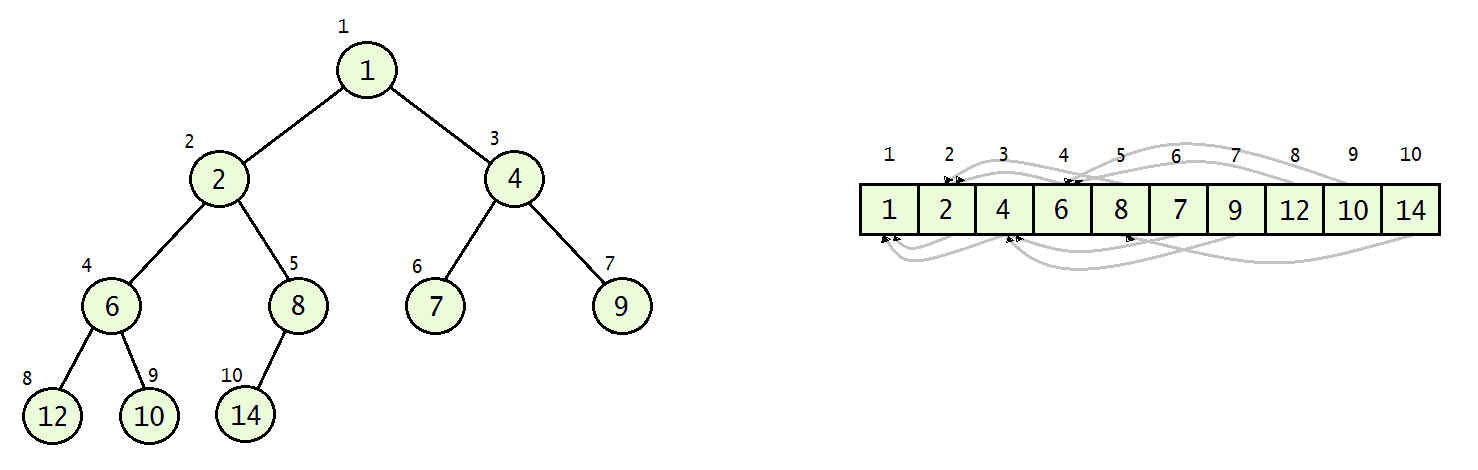
\includegraphics[scale=0.4]{Pictures/Heap and array.png}
\caption{Min-heap seen as a binary tree and an array.}
\end{figure}

\noindent By using the properties of the binary heap, we can compute the parent and left/right child of a node, given its index by:\\
%\begin{center}
%$$\pmb{Parent(i) = \lfloor i/2 \rfloor}$$\\
$$Parent(i) = \lfloor i/2 \rfloor$$
%\pmb{$Left(i) = 2i$}\\
$$Left(i) = 2i$$
%\pmb{$Right(i) = 2i+1$}\\
$$Right(i) = 2i+1$$
%\end{center}

\ \\In the binary min-heap we have that the value of the nodes are in decreasing order when moving from a leaf node, up through the parent-nodes. Symmetrically, we have that the values are in ascending order when moving down arbitrarily through the nodes. That is, we have for all nodes that Min-heap[Parent(i)] $\leq$ Min-heap[i].\\

\noindent For our shortest-path algorithms to work on the binary heap datastructure, we need the following operations:

\newpage
\subsection{Decrease-Key}
When updating the min-heap, we use the Decrease-Key method, which decreases the value of a given node $i$, if our relaxation can improve the distance-estimate. The pseudocode can be seen below:\\

\textbf{DECREASE-KEY(Min-Heap, i, key)}
\begin{enumerate}
\NumTabs{24}
\setlength\itemsep{0em}
\item Min-Heap[i] = key
\item \textbf{while } i $>$ 1 and Min-Heap[Parent(i)] $>$ Min-Heap[i]
\item \tab{Swap(Min-Heap[i], Min-Heap[Parent(i)])}
\item \tab{i = Parent(i)}
\end{enumerate}

\noindent The method changes the value of node $i$ to our key and as long as the Parent($i$) is larger than $i$, it swaps $i$ with Parent($i$), and assigns the value of $i$ to Parent($i$).\\


\subsection{Insert}
Insertion is the method of inserting a new node into our Min-Heap. Its pseudocode is seen below:\\

\textbf{INSERT(Min-Heap, key)}
\begin{enumerate}
\NumTabs{24}
\setlength\itemsep{0em}
\item Size(Min-Heap) = Size(Min-Heap) + 1
\item Min-Heap[Size(Min-Heap)] = NIL
\item DECREASE-KEY(Min-Heap, Size(Min-Heap), key)
\end{enumerate}

\noindent When we insert, we increase the size of our heap by 1, and insert it at the end. We also make a call to Decrease-Key to have the new node be at the right place in the Min-Heap.\\

\noindent We can in the ordinary Dijkstra's algorithm do this in a more clever way which will be discussed in section~\ref{sec:clever}.
\subsection{Extract-Min}
By calling our Extract-Min we take out the Min-Heap[1], which is the root of our Min-Heap and the new root will be guaranteed, by the call to Balance-Min-Heap, to have the minimum value. The pseudocode is for Balance-Min-Heap and Extract-Min can be seen here:\\

\textbf{BALANCE-MIN-HEAP(Min-Heap, i)}
\begin{enumerate}
\NumTabs{24}
\setlength\itemsep{0em}
\item L = Left(i)
\item R = Right(i)
\item \textbf{if } L $\leq$ Size(Min-Heap) \textbf{and} (Min-Heap[L] $<$ Min-Heap[i])
\item \tab \textbf{then } smallest = L
\item \tab \textbf{else } smallest = i
\item \textbf{if } R $\leq$ Size(Min-Heap) \textbf{and} (Min-Heap[R] $<$ Min-Heap[smallest])
\item \tab \textbf{then } smallest = R
\item \textbf{if } smallest $\neq$ i
\item \tab \textbf{then } Swap(Min-Heap[i], Min-Heap[smallest])
\item \tab \tab BALANCE-MIN-HEAP(Min-Heap, smallest)
\end{enumerate}

\noindent Balance-Min-Heap takes a Min-Heap and the index of a node and then balances the heap. This is done by swapping the node with its smallest child-node recursively, until the key of both child-nodes are greater than or equal to the node's key. If the key of left child node is smaller than $i$, we set the smallest to be the left node, otherwise we set it to $i$ (line 3-5). Next, we do a second check on whether the right child is smaller than the current smallest node. If true, we set the right child to be the smallest (line 6-7). Then, we check if the smallest is not $i$. If true, we swap it with the smallest node and call Balance-Min-heap with the new smallest node's index (line 8-10).\\\\


\textbf{EXTRACT-MIN(Min-Heap)}
\begin{enumerate}
\NumTabs{24}
\setlength\itemsep{0em}
\item \textbf{if } Size(Min-Heap) $<$ 1
\item \tab raise error "Heap underflow"
\item min = Min-Heap[1]
\item Min-Heap[1] = Min-Heap[Size(Min-Heap)]
\item Size(Min-Heap) = Size(Min-Heap) - 1
\item BALANCE-MIN-HEAP(Min-Heap, 1)
\item \textbf{return} min
\end{enumerate}

\noindent Extract-Min saves the root into the variable min. Afterwards, it puts the terminal node up in the root and decreases the heap-size by 1. Then it makes a call to Balance-Min-Heap to balance the tree, and returns the root node contained in min.


\newpage
%%%%%%%%%%%%%%%%%%%%%%%%%%%%%%% Dijkstra %%%%%%%%%%%%%%%%%%%%%%%%%%%%%%%
\section{Dijkstra's algorithm}
Dijkstra's algorithm takes a weighted graph $G = (V, E)$ and finds the shortest path from a single source to each other vertex in the graph. To keep track of the vertices, the algorithm maintains two sets of vertices. The set $S$ consists of vertices, where the optimal shortest-path estimate from the source $s$ has been figured. The other set $Q$ is a minimum priority queue that contains the remaining vertices, i.e. $Q = V - S$. The algorithm will repeatedly extract a vertex with the minimum shortest-path estimate from $Q$ and add it to $S$, until all vertices have been discovered. If the graph happens to be connected, then for all $v \in V $, a vertex $v$ will be reachable from another vertex $w$ through an edge. If the graph is disconnected, some vertices will be unreachable, thus making some shortest paths infinite, if we try to reach these vertices.\\

\noindent 
\textbf{Assumptions}\\
For Dijkstra's algorithm to work, we must assume that the graph contains no negative weights. Once a vertex has been extracted from the min-priority queue, Dijkstra's algorithm will assume that the shortest path to that vertex has been found. This means the algorithm will never have to relax this vertex again. However, if there is a negative-weighted edge somewhere, the algorithm may find a wrong shortest-path.\footnote{"Why doesn't Dijkstra's algorithm work for negative weight edges", Amit, stackoverflow.com}An example can be seen in the following figure:\\

\begin{figure}[H]
\centering
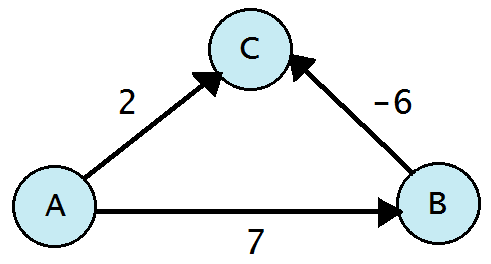
\includegraphics[scale=0.3]{Pictures/Dijkstra - no negative weight.png}
\caption{A graph with negative weights.}
\end{figure}

\noindent In this figure, the graph consists of three vertices $A, B,$ and $C$. Dijkstra's algorithm starts at the source $A$ and will first extract $C$, since it has the shortest-path estimate of 2. Afterwards, the algorithm extracts the last vertex $B$ and terminates. Had it however tried to relax the negative edge between $B$ and $C$, a shorter path of $7 - 6 = 1$ would have been discovered. The result is therefore incorrect due to Dijkstra's algorithm utilizing the greedy property of the triangle inequality, thus that $\forall (u,v) \in E.(w(u,v) \geq 0)$. \\

\noindent The pseudocode for Dijkstra's algorithm can be seen below:\footnote{Introduction to Algorithms, pg. 658}
\subsection{Pseudocode for Dijkstra's algorithm}

\hspace{4ex}\textbf{DIJKSTRA$(G, w, s)$}
\begin{enumerate}
\NumTabs{24}
\setlength\itemsep{0em}
\item INITIALIZE-SINGLE-SOURCE$(G, s)$
\item $S = $ \O
\item $Q = G.V$
\item $\textbf{while } Q \neq$ \O
\item \tab{$u = $ EXTRACT-MIN$(Q)$}
\item \tab{$S = S \cup \{u\}$}
\item \tab{\textbf{for} each vertex $v \in G.Adj[u]$}
\item \tab{}\tab{RELAX$(u,v,w)$}
\end{enumerate}

\noindent The graph is initialized in line 1 by calling INITIALIZE-SINGLE-SOURCE. For each vertex $u \in V$, the function sets the shortest-path estimate to $\infty$ and predecessor to NIL. $d[s]$ is set to 0. Dijkstra's algorithm maintains two sets, $S$ and $Q$. The set $S$ contains the vertices, whose final shortest-path estimates have been determined. In the beginning, no paths have been determined and thus $S$ will be empty (line 2). The min-priority queue $Q$ contains the vertices, whose shortest paths have not been found yet and is keyed by the vertices' current shortest-path estimates. In other words, the set of vertices in the graph is equal to the two sets, $V = S + Q$. At start, $Q$ will contain all vertices in the graph (line 3).\\

\noindent We want to find the shortest-path estimate $d[u]$ for all vertices, so Dijkstra's algorithm runs until the priority queue is empty. While $Q$ is not empty, the algorithm extracts the vertex with lowest $d[u]$ from $Q$ and adds it to the set $S$ (line 4 to 6). Afterwards, we examine for each vertex $v$ adjacent to $u$ if the shortest path found so far can be enhanced by taking the path through $u$. This is done by relaxing the edge $(u,v)$ (line 7 to 8).\\


%%%%%%%%%%%%%%%%%%%%%%%%% Dijkstra  modified %%%%%%%%%%%%%%%%%%%%%%%%%
\subsection{Dijkstra's algorithm - modified}
\noindent The original pseudocode finds the shortest path from a source vertex to all other vertices. We are only interested in finding the shortest path for a single target, so we have therefore modified the original pseudocode for Dijkstra's algorithm. As soon as the algorithm finds the shortest path to the target vertex, it will terminate. This will reduce the amount of vertices visited, unless the target happens to be the last vertex found.\\
\subsubsection{Pseudocode for modified Dijkstra's algorithm}
\hspace{4ex}\textbf{MODIFIED-DIJKSTRA$(G, w, s, t)$}
\begin{enumerate}
\NumTabs{24}
\setlength\itemsep{0em}
\item $d[s] = 0$
\item $S = Q = \{s\}$
\item $\textbf{while } Q \neq  $ \O
\item \tab{$u = $ EXTRACT-MIN$(Q)$}
\item \tab{\textbf{if } $u = t$}
\item \tab{}\tab{\textbf{Terminate}}
\item \tab{\textbf{for} each vertex $v \in G.Adj[u]$}
\item \tab{}\tab{\textbf{if } $v \notin S$}
\item \tab{}\tab{}\tab{$S = S \cup \{v\}$}
\item \tab{}\tab{}\tab{$Q = Q \cup \{v\}$}
\item \tab{}\tab{}\tab{$d[v]  = d[u] + w(u,v)$}
\item \tab{}\tab{}\tab{$\pi[v] = u$}
\end{enumerate}

\noindent The pseudocode now takes a 4th parameter $t$, indicating the target vertex we want to find. Instead of calling the function \textit{INITIALIZE-SINGLE-SOURCE}, we only set the source's shortest-path estimate to 0. All other vertices are already assumed to have a shortest-path estimate equal to $\infty$, so it is not necessary to initialize the estimates to $\infty$.\\

\noindent The set $S$ no longer contains the vertices, whose final shortest-path estimates have been found. Instead, the set $S$ now consists of vertices $u$ for which a path to $u$ has been considered. By subtracting $S$ from $V$, we would get the set of vertices that originally would be $d[u]=\infty$. The min-priority queue $Q$ has also been modified. Instead of adding all vertices in the graph, we only want to insert new vertices into the queue as they are discovered.\\ 

\noindent At start, $s$ is added to the sets $S$ and $Q$, since only the path to the source has been discovered and considered (line 2). Line 4 extracts a vertex $u$ with the minimum shortest-path estimate. If the vertex $u$ is the target vertex, the algorithm terminates. Otherwise, the algorithm examines each vertex $v$ that is adjacent to $u$ in line 7. If $v$ has not been examined before, it will not be an element of $S$ or $Q$. Thus, we add $v$ to $S$ and $Q$. After this, the edge $(u,v)$ is relaxed, since $d[v]=\infty$ prior to being found and the predecessor is then set to $u$.\\\\
The following figure illustrates the difference between the two algorithms.\\
\begin{figure}[H]
\centering
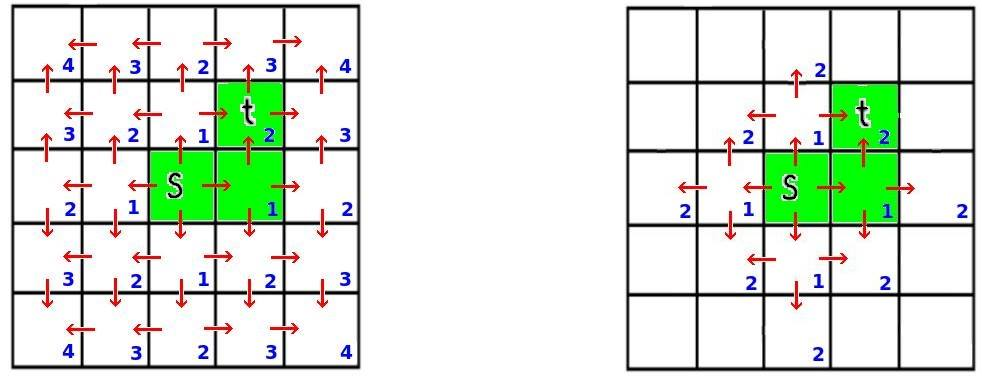
\includegraphics[scale=0.4]{Pictures/Comparison0.jpg}
\caption{Dijkstra's algorithm vs. the modified Dijkstra's algorithm.}
\end{figure}

\noindent In this figure, the tiles illustrate vertices and the red arrows illustrate the edges that have been relaxed. The green tiles indicate the vertices in the shortest path from $s$ to $t$. It is seen that the original Dijkstra's algorithm relaxes all edges in the graph, while the modified algorithm only relaxes until the target has been found. Thus, the modified Dijkstra's algorithm terminates earlier in this example.


%%%%%%%%%%%%%%%%%%%%%%%%%%%% Dijkstra proof %%%%%%%%%%%%%%%%%%%%%%%%%%%%
\subsection{Correctness of Dijkstra's algorithm}
To prove that Dijkstra's algorithm works, we will perform an induction proof. Let $S$ be the set of vertices, whose shortest path have been found, $S=V-Q$.\\

\noindent \textbf{Loop Invariant}\\
$\forall v\in S.(d[v] = \delta(s,v))$\\

\noindent \textbf{Initialization}\\
Let Size$(S)=1$. This is true when $S$ only holds the source vertex, $S = \{s\}$. Since $d[s]=0=\delta(s)$, the invariant holds.\\

\noindent \textbf{Maintenance}\\
Let $v$ be the latest vertex added to $S$. Let $S'$ = $S \cup \{v\}$. For each vertex in $S'$, we want to have that our loop invariant holds. EXTRACT-MIN(Q) ensures that the correct distance label gets extracted from $Q$ and put into $S$. We therefore only need to show that $d[v]=\delta(s,v)$ for $S'=S \cup \{v\}$. To prove this, we will perform a contradiction. Assume that there exists a shortest path $P^{sv}=\{s, ..., v\}$ from the source vertex $s$ to target vertex $v$ that has length $$w(P^{sv}) < d[v]$$
Before adding $v$ to $S$, the path $P^{sv}$ connects a vertex $u\in S$ to the vertex $v\in V-S$ through one or more edges. Since $v$ has not been added to $S$ yet, there must be one or more vertices on the path $P^{sv}$ that is in $V-S$. And since the source $s$ is in $S$, there must be one or more vertices on the path $P^{sv}$ that belongs to $S$. We can therefore define a vertex $y$ to be the first vertex along $P^{sv}$ that is an element of $V-S$. Let $x\in S$ be $y's$ predecessor along the path $P^{sv}$. Let $P^{sx}=\{s, ..., x\}$ be a subpath of $P^{sv}$ from vertex $s$ to $x$. This path is illustrated on figure~\ref{fig:eyy}. Since $x \in S$, we know by induction that $x$ got extracted with the correct shortest path distance $$d[x] \leq w(P^{sx})$$and that the edge $(x,y)$ got relaxed, so $$d[y]$$$$\leq d[x]+w(x,y)$$$$\leq w(P^{sx}) + w(x,y)$$$$\leq w(P^{sv})$$But we assumed $w(P^{sv}) < d[v]$ and $d[y] < d[v]$, which contradicts that EXTRACT-MIN returns a vertex $v$ from $V-S$ minimizing $d[v]$. $v$ has the shortest distance label, so $$d[v] \leq d[y]$$

\noindent \textbf{Termination}\\
We terminate once $Q = V-S =\O$. If $\exists t \in S$, we can backtrace the predecessors to obtain $\delta(s,t)$. Otherwise, we have that $\delta(s,t) = \infty$ by the no-path property.\\

\begin{figure}[H]
\centering
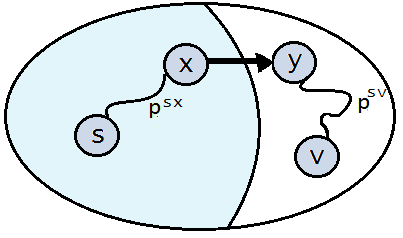
\includegraphics[scale=0.5]{Pictures/Dijkstra - Proof of correctness.png}
\caption{Proof of correctness.}
\label{fig:eyy}
\end{figure}

\noindent The figure shows an assumed shorter path $p^{sv}$ from source vertex $s$ to vertex $v$, decomposed into $s\rightsquigarrow x\rightarrow y \rightsquigarrow v$. Vertex $y$ is the first vertex along the path that is an element of $V-S$ (white area). Vertex $x$ is y's predecessor and an element of $S$ (blue area). It is possible that $s=x$ or $y=v$.

%%%%%%%%%%%%%%%%%%%%%%%%%%%%%%% A* search %%%%%%%%%%%%%%%%%%%%%%%%%%%%%%%
\newpage
\section{A* search}
The A* search algorithm was developed in 1968 and can be seen as a mix of Dijkstra's algorithm and Greedy Best-First search algorithm. 

\subsection{Utilization of Dijkstra's algorithm and Greedy Best-First search}
\noindent A* search algorithm works similar to Dijkstra's algorithm in that it examines an edge only once, and will favor vertices who are close to the source vertex. This means that it examines the vertices with the smallest shortest-path estimates first. The downside of Dijkstra's algorithm is however that the target vertex' direction is unknown. Thus, Dijkstra's algorithm might consider paths going in the complete opposite direction. Instead, A* search uses heuristics to guide its search in a more precise direction. The heuristic function can estimate how far away any vertex is from the goal. Vertices close to the goal are then favored over vertices who lie far away. By using heuristics, A* search is similar to the Greedy Best-First search algorithm that also uses heuristics.\\

\noindent The Greedy Best-First search algorithm is a pure heuristic algorithm that searches for a path between two vertices by using only the heuristic as information. When expanding a path, it favors the vertex closest to the goal. By making a greedy decision based on one criterion, the Greedy Best-First search algorithm runs considerably faster than Dijkstra's algorithm. Greedy Best-First search can however not guarantee a shortest path, which is illustrated in the following example:

\begin{figure}[H]
\centering
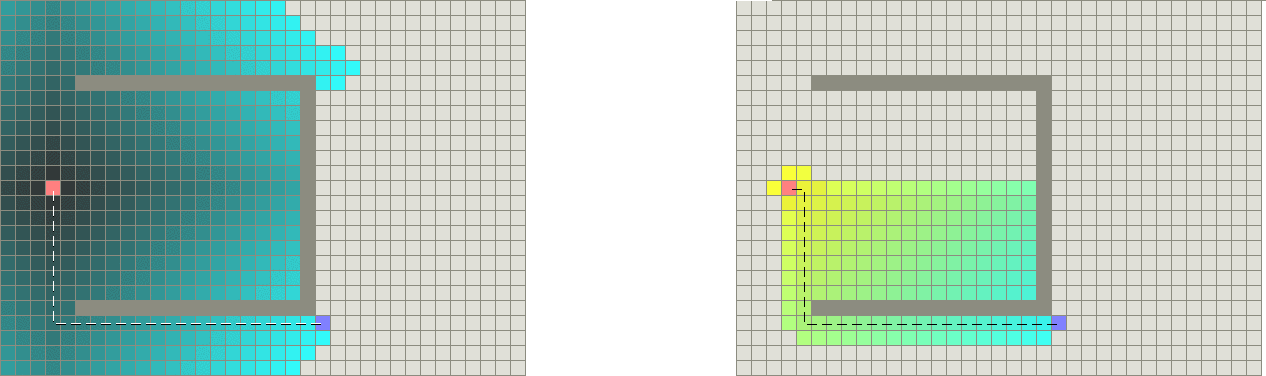
\includegraphics[scale=0.45]{Pictures/Comparison2.png}
\caption[]{Dijkstra's algorithm  vs  Greedy Best-First search.\footnotemark}
\end{figure}
\footnotetext{Amit P, Introduction to A*}

\noindent In this figure, Dijkstra's algorithm is seen to the left and Greedy Best-First search to the right. The pink square represents the source vertex, while the dark blue square represents the target vertex. The other colored squares are vertices who have been visited. Between the source and target, there is a grey border indicating an obstacle that the path cannot go through.\\ 

\noindent In the example, it is seen that Dijkstra's algorithm expands in all directions until it ultimately finds a shortest path to the target. Meanwhile, Greedy Best-First search expands over less vertices since the heuristic function leads its way, making it run faster than Dijkstra's algorithm. However, Greedy Best-First search found a path that was not a shortest path. The path moves toward the corner of the obstacle and then has to navigate around the obstacle before finding the target. By ignoring the distance moved so far, the Greedy Best-First search algorithm continues on the path it is on, even when the path has become very long.\\

\noindent A* search does not perform a pure heuristic search, since it keeps the estimated distance from source to vertex in mind, before extending the path. A* search will therefore not be as fast as Greedy Best-First search, but will at least guarantee that a shortest path is found, if we use an admissible heuristic function. This will be explained in the following subsection. By combining the information that Dijkstra's algorithm and Best-First search uses, A* search will be at least as fast as Dijkstra's algorithm, since the search can go in a more precise direction. This makes us able to minimize the number of vertices visited, before the target vertex is found. \\

%%%%%%%%%%%%%%%%%%%%%%%%%%%%%% Heuristics %%%%%%%%%%%%%%%%%%%%%%%%%%%%%%
\subsection{Heuristic function for A* search}
A* search will behave differently, depending on which heuristic function $h(v)$ we take in use. In the special case where $h(v)$ always gives 0, then only the shortest path estimate $d[v]$ will be looked at when a node is expanded. In this case, A* search will be equal to Dijkstra's algorithm, since Dijkstra's algorithm only considers $d[v]$. On the other hand, if $h(v)$ happens to be very high compared to $d[v]$, then only $h(v)$ is important. Thus, A* search turns into Greedy Best-First search and become a pure heuristic algorithm.\footnote{"Heurestics", Amit, stanford.edu}\\

\noindent If $h(v)$ is always smaller than or equal to the cost of moving from a vertex $v$ to the goal, then A* search is assured to find a shortest path. When the  heuristic function $h(v)$ never overestimates the cost, the heuristic function is said to be admissible. An admissible heuristic can be seen as being too optimistic. It will make A* search consider paths that are more costly than the shortest path. The smaller $h(v)$ is, the more nodes A* search will expand, since the heuristic function is guiding the search in a less precise manner. It is therefore preferable to make $h(v)$ be as close as possible to the exact cost of moving from a vertex to the goal, since A* search will expand less nodes and run faster. \footnote{"CS440: Introduction to Artificial Intelligence", C. Anderson, colostate.edu}\\

\noindent In the case where $h(v)$ is not admissible and overestimates the cost of moving from a vertex $v$ to the goal, A* search can not guarantee to find a shortest path. On the other hand, A* can run even faster, since the search will be more specific, making A* search expand less nodes. This property can for example be useful in games. If a computer is slow, computing a good path quickly may be preferable over computing an ideal path slowly.\\

\noindent Suppose we have a game, where the goal can be reached from going through a forest or flat land, and that the movement cost is 3 for the forest and 1 for flat land. A* search thus expands over flat land three times as much as over the forest. If we for example decrease the movement cost on the forest from 3 to 2, A* search will only expand twice as far along the flat land, compared to the forest. The shortest path will not be found, but on the good side we have increased the speed at which A* search computes. \footnote{"Heurestics", Amit, stanford.edu}\\\\

\noindent \textbf{The Euclidean distance:}\\
\noindent The heuristic function we chose to use for A* search, takes a vertex $v \in V$ and the destination vertex $t \in V$, and computes the Euclidean (i.e. straight-line) distance from $v$ to $t$. The Euclidean distance in a n-dimensional space on points $v$ and $t$ is computed by the following formula:\\
$$\sqrt{\displaystyle\sum_{i=1}^{n} (v_i - t_i)^2}$$
As we primarily consider plannar graphs, the Euclidean distance will be implemented using 2 dimensions, thus:\\
$$\sqrt{(v_x - t_x)^2 + (v_y - t_y)^2}$$
By using the Euclidean distance as our heuristic, we can guarantee that $h(v)$ will always be admissible. This is proved in section $10.4$.


%%%%%%%%%%%%%%%%%%%%%%%%% Pseudocode - A* search %%%%%%%%%%%%%%%%%%%%%%%%%
\subsection{Pseudocode for A* search algorithm}
We wish to find the shortest path to a single target, so the pseudocode is based on the pseudocode for the modified Dijkstra's algorithm.\\

\textbf{A* search$(G, w, s, t)$}
\begin{enumerate}
\NumTabs{24}
\setlength\itemsep{0em}
\item $d[s] = 0$
\item $S = Q = \{s\}$
\item $\textbf{while } Q \neq  $ \O
\item \tab{$u = $ EXTRACT-MIN$(Q)$}
\item \tab{\textbf{if } $u = t$}
\item \tab{}\tab{\textbf{for }each vertex $v \in S$}
\item \tab{}\tab{}\tab{$d[v] = \infty$}
\item \tab{}\tab{\textbf{Terminate}}
\item \tab{\textbf{for} each vertex $v \in G.Adj[u]$}
\item \tab{}\tab{\textbf{if } $v \notin S$}
\item \tab{}\tab{}\tab{$S = S \cup \{v\}$}
\item \tab{}\tab{}\tab{$Q = Q \cup \{v\}$}
\item \tab{}\tab{}\tab{$d[v]  = d[u] + w(u,v)$}
\item \tab{}\tab{}\tab{$\pi[v] = u$}
\item \textbf{for} each vertex $v \in S$
\item \tab{$d[v] = \infty$}
\end{enumerate}
Like the modified Dijkstra's algorithm, A* search algorithm maintains two sets $S$ and $Q$. The set $S$ contains vertices $v$, for which a path to $v$ has been considered. As new vertices are discovered, they are also added to the min-priority queue $Q$. After adding a vertex $v$ to $S$ and $Q$, we then relax the edge and update the predecessor. To make sure that edges are relaxed properly, A* search may only take non-negative edges.\\

\noindent Recall that Dijkstra's algorithm selects which vertex to visit next, by extracting the vertex with the lowest shortest-path estimate, $d[v]$ in the priority queue. The difference between Dijkstra's algorithm and A* search is that we now use heurestics to guide our search. A* search's min-priority queue is keyed by the current shortest path estimate $d[v]$ for each vertex $v$, added with the heuristic function $h(v)$. Each time A* search algorithm chooses which vertex to extract, it extracts the vertex $v$ with the lowest sum $d[v]+h(v)$.\\

\noindent  The heuristic estimated cost $h(v)$ that we examine, is gotten by taking the Euclidean distance from a vertex $v$ to the target vertex $t$. By repeatedly selecting the vertex with the lowest sum, we can get a more precise path search. This is illustrated in the following figure:\\

\begin{figure}[H]
\centering
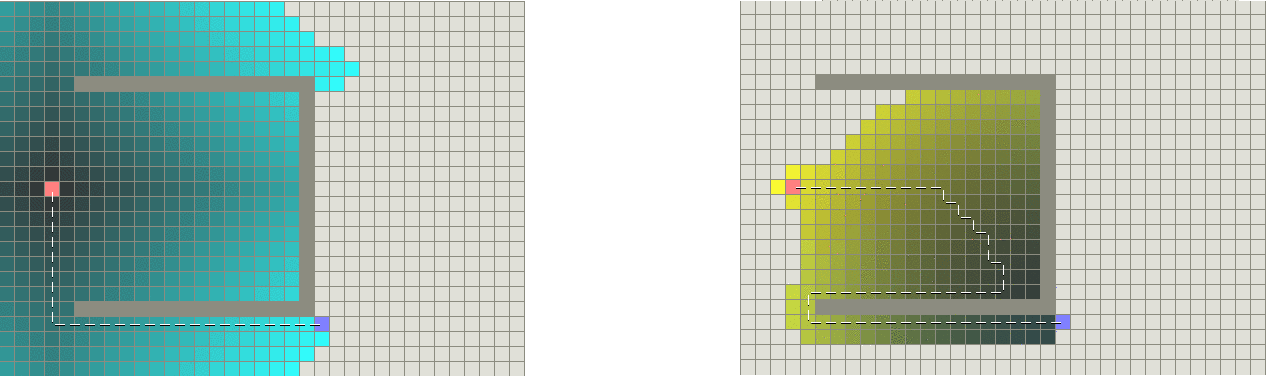
\includegraphics[scale=0.45]{Pictures/Comparison1.png}
\caption[]{Dijkstra's algorithm  vs  A* Search algorithm.\footnotemark}
\end{figure}
\footnotetext{Amit P, Introduction to A*}

\noindent In this figure, the pink square represents the source vertex, while the dark blue square represents the target vertex. The other colored squares represent vertices who have been visited. Dijkstra's algorithm to the left has no estimation of how far away any vertex is, and thus expands in every direction, when trying to compute the shortest path to target. Meanwhile, A* search keeps the Euclidean distance to the target in mind and thus favors vertices who lie south-east from the starting point. This roughly reduces the amount of vertices visited by half in the example, making A* search much more efficient.\\

\noindent The A* search algorithm provides the heuristic to embed additional knowledge directly into a formal mathematical search process. For example, people who use automated programs that compute a shortest path, such as Google Maps, often have to modify results derived by the formal method in order to take advantage of additional "informal" sources of knowledge.\footnote{Encyclopedia of Artificial Intelligence Volume 1 A-L, pg. 1, Shapiro, Raphael B.} E.g. if you're on a bicycle and want to travel home, Google Maps may suggest you move along the short, but muddy terrain through the forest. Instead, you may choose a longer route, bypassing the forest, since the path Google suggested will actually take a longer time to pass due to the muddy terrain. 

%%%%%%%%%%%%%%%%%%%%%%%%%%%% A* search proof %%%%%%%%%%%%%%%%%%%%%%%%%%%%
\subsection{Correctness of A* search algorithm}
To prove that A* search algorithm work, we will perform an induction proof. Let $S$ be the set of vertices, whose path have been considered. Let $d[v]$ be the shortest path estimate from the source to vertex $v$. Let $h(v)$ be the heurestic function that returns the Euclidean distance from vertex $v$ to target vertex.\\

\noindent \textbf{Loop Invariant}\\
For a shortest path $P={s, v_1, ..., t}$ from source vertex to target vertex, $\forall v \in P$ we have that $d[v] = \delta(s,v)$.\\

\noindent \textbf{Initialization}\\
Let Size$(S)=1$. This is true when $S$ only holds the source vertex, $S = \{s\}$. Since $d[s]=0=\delta(s)$, the invariant holds.\\

\noindent \textbf{Maintenance}\\
Let $v$ be the last vertex added to $S$. Let $S'$ = $S \cup \{v\}$. For each vertex in $S'$ that is on the path $P$, we want to have that our loop invariant holds. This holds true if the heuristic is admissible and if $\forall v \in P$ we have that $d[v]=\delta(s,v)$. EXTRACT-MIN(Q) ensures that the smallest sum of $d[v]+h[v]$ gets extracted from $Q$ and put into S. We therefore only need to show that $h(v)$ is admissible and that $d[v]=\delta(s,v)$ for the vertices in $S'$ that is on the path $P$. To prove this we will perform two proofs by contradiction, one for $h(v)$ and the other for $d[v]$.\\

\noindent Let the heuristic function be the Euclidean distance from a vertex $u$ to $v$, $h(v)=\|(u,v)\|$. Assume that there exists a path from $u$ to $v$ through a vertex $x$ that is less than the distance measured from $u$ to $v$. Thus, the heuristic function will have overestimated the distance from vertex v to target $t$. Since we measure the Euclidean (straight-line) distance, this can be seen as a triangle, where $$\|(u,v)\| > \|(u,x)\| + \|(x,v)\|$$\textbf{Lemma:} For any triangle, with sides $\{u,v,x\}$ we have that $\|v\| \leq \|u\| + \|x\|$.\\ 

\noindent From this lemma we have that any side of the triangle must be less than or equal to the sum of the remaining sides. But since we assumed that $\|(u,v)\| > \|(u,x)\| + \|(x,v)\|$ we must not have a triangle, and thus, we would have a wrong measurement for $\|(u,v)\|$. This is in contradiction with the original assumption that we had the Euclidean distance $\|(u,v)\|$, and thus $$\|(u,v)\| \not > \|(u,x)\| + \|(x,v)\|$$
We can now derive that $$\|(u,v)\| \leq \|(u,x)\| + \|(x,v)\|$$which contradicts that we had a path from vertex u to v through x that would be less than $\|(u,v)\|$. Thus we have that the Euclidean distance from $u$ to $v$ is measured correctly and that the heuristic function $h(v)$ is admissible.\\

\noindent For the next proof by contradiction, assume that there exists a shortest path $P^{sv}=(s, ..., v)$ from the source vertex $s$ to target vertex $v$ that has length $$w(P^{sv}) < d[v]$$
Before adding $v$ to $S$, the path $P^{sv}$ connects a vertex $u\in S$ to the vertex $v\in V-S$ through one or more edges. Since $v$ has not been added to $S$ yet, there must be one or more vertices on the path $P^{sv}$ that is in $V-S$. And since the source $s$ is in $S$, there must be one or more vertices on the path $P^{sv}$ that belongs to $S$. We can therefore define a vertex $y$ to be the first vertex along $P^{sv}$ that is an element of $V-S$. Let $x\in S$ be $y's$ predecessor along the path $P^{sv}$. Let $P^{sx}=(s, ..., x)$ be a subpath of $P^{sv}$ from vertex $s$ to $x$. Since $x \in P$, we know by induction that $x$ has the correct shortest path distance $$d[x] + h(x) \leq w(P^{sx}) + h(x)$$and that the edge $(x,y)$ got relaxed, so $$d[y]+h(y)$$ 
$$\leq \; d[x]+w(x,y)+h(y)$$
$$\leq \; w(P^{sx}) + w(x,y) + h(y)$$
$$\leq \; w(P^{sv})$$But we assumed $w(P^{sv}) < d[v]$ and $d[y] < d[v]$, which contradicts that EXTRACT-MIN returns a vertex $v$ from $V-S$ with the minimum $d[v]+h(v)$. $v$ has the shortest distance label, so $$d[v] \leq d[y]$$
\textbf{Termination}\\
We terminate once target $t$ has been found or $Q = V-S =\O$. If $\exists t \in S$, we can backtrace the predecessors to obtain $\delta(s,t)$. Otherwise, we have that $\delta(s,t) = \infty$ by the no-path property.\\


%%%%%%%%%%%%%%%%%%%%%%%%% Implementation %%%%%%%%%%%%%%%%%%%%%%%%%%
\section{Implementation}
To examine the complexity of Dijkstra's algorithm, Bellman-Ford, and A* search algorithm, we have implemented them in C++. The code can be found in the appendix and also on our GitHub page: \url{https://github.com/Pjuske/Bachelors-Thesis}. We have used the following C++ libraries in our implementations:\footnote{C++ Reference, cplusplus.com}

\begin{itemize}
\item $<$vector$>$
\item $<$queue$>$
\item $<$set$>$
\item$<$climits$>$
\item $<$fstream$>$
\item$<$ctime$>$
\item $<$iostream$>$
\end{itemize}

\noindent The $<$vector$>$ library allows us to define vectors that represent arrays that can change in size. With vectors, adding or removing elements from its end is quite efficient. This is for example useful for saving predecessor pairs. When an algorithm discovers a new vertex, we want to save a new vector containing the vertex and its predecessor. Since the number of vertices discovered will vary from target to target, a dynamic array will therefore be useful.\\

\noindent For the implementation of Dijkstra's algorithm and A* search algorithm, we used the $<$queue$>$ library to make a priority queue that contains pairs of integers. To store the pairs, we use the library $<$set$>$ that allows us to store the elements so they follow a certain order.\\

\noindent For the implementation of Bellman Ford, we needed to initialize the distance of all vertices to $\infty$. This was done by using the library $<$climits$>$ to set their distances to the maximum integer value in C++. By doing this, we will know that a vertex has been visited if its distance is less than the maximum value.\\

\noindent The library $<$fstream$>$ made reading and writing to files possible. We used the library to write graph information into text files. The algorithm implementations then read these files and used the information to create a graph. This is described in further detail in the subsection 'implementation of graphs'.\\

\noindent When the implementations were finished, we wanted to measure the processor time for each algorithm by using the library $<$ctime$>$. By calculating the difference between the start and termination of our program execution, we can get the runtime for each algorithm in milliseconds. To print the time taken, as well as the shortest path and total distance, we used the library $<$iostream$>$. Pictures of the output can be seen in our appendix.\\

\noindent To show the shortest path, we made a function print\textunderscore path() that prints the path taken from source to target vertex. The following pseudocode PRINT-PATH illustrates how print\textunderscore path() works:\footnote{Introduction to Algorithms, pg. 601, CLRS}

\newpage
\noindent \textbf{PRINT-PATH$(G, s, v)$}
\begin{enumerate}
\NumTabs{24}
\setlength\itemsep{0em}
\item \textbf{if }$v == s$
\item \tab{print $s$}
\item \textbf{elseif }$v.\pi == NIL$
\item \tab{print "no path from $s$ to $v$ exists"}
\item \textbf{else } PRINT-PATH$(G, s, v.\pi)$
\item \tab{print $v$}
\end{enumerate}

\noindent The algorithm takes a graph $G$, source $s$, and target vertex $v$ as arguments. If target is equal to source, the source is printed. If $v$ has no predecessor, we print that no path from $s$ to $v$ exists. Else, we print the target $v$ and run the algorithm recursively, giving $v$'s predecessor as the target. The algorithm will then run until the predecessor is equal to the source.\\

\subsection{Implementation of graphs}
\noindent We received four text files with sample graphs of increasing size (vertices = $41, 160, 638, 2542$) from one of our tutors. The sample graphs contained the coordinates $(x,y)$ of each vertex, and information about which vertices were connected by an edge. To get the edge weight for each edge in a graph, we would then read the file inside a C++ program we made, called 'graph-converter.cpp'.\\ 

\noindent The converter receives information about how many vertices and edges the graph contains, as well as what vertex we choose as target. It then proceeds to calculate all the edge weights by computing the Euclidean distance between the connected vertices. After this, the converter writes the result into a new file, e.g. "data{\_}0.txt" where each line is of the form $(u, v, w)$. $u$ is the predecessor to $v$ and $w$ is the edge weight between $(u,v)$.\\

\noindent After writing the information about vertices and edge weights, we then compute the Euclidean distance to the target for each vertex in the graph. This gives us our heuristic function $h(v)$ that the implementation of A* search takes in use. These values are also written to the same file. Thus each of our three implementations only have to open one file and extract the information they each need.\\

\noindent The implementations then use the new file to create the graph. The graph is a vector array of tuples, where the index is equal to a vertex $u$, and its tuples contains information about the weight and successor of that vertex, which is why the new file contains data of form $(u,v,w)$. For example if vertex $u=1$ is connected to vertex $2$ and $3$ by weight $10$ and $20$, we can use the function push{\_}back() to add the tuple values:
$$graph[1].push{\_}back(id(2, 10))$$
$$graph[1].push{\_}back(id(3, 20))$$ 

\subsection{Implementation of Bellman Ford algorithm}
The implementation of Bellman Ford algorithm has two vector arrays containing the graph and predecessor information. It also has an array containing the distance to source for each vertex $v\in V$. Furthermore, we also have a variable that counts how many times the algorithm visits an edge.\\

\noindent The Bellman Ford function takes the number of vertices in graph and the source vertex as arguments. It then initializes the graph by setting all distances to $\infty$, except for the source that has distance $0$. Afterwards, it runs a loop $G|V| - 1$ times. For each iteration, it goes through all the vertices and look at the edges coming out from each vertex. Every time we find an edge, we increase the variable that counts number of edge-lookups by 1. We then relax each edge $(u,v)$ from a vertex $u$ to $v$ and update the distance array if the distance can be improved. If vertex $v$ has no predecessor, we insert $u$ into the predecessor array. Otherwise, we overwrite the former predecessor with $u$ inside the predecessor array.\\

\noindent After the iterations, we go through the graph and check for negative-weight cycles. If found, the program returns false, otherwise true. When the program has terminated, we measure the runtime, and print it to the terminal along with the path, distance, and amount of edge lookups.

\subsection{Implementation of Dijkstra's algorithm}
The implementation for the modified Dijkstra's algorithm keeps a graph and predecessor vector array, plus a distance array and a variable counting edge-lookups. We also have an array that stores information about which vertices have been visited yet. Instead of initializing all vertices to have $d[v]=\infty$, we thus only need to update the distances and mark the vertices as visited as we discover them. This should make the program run faster.\\

\noindent The Dijkstra's algorithm function takes the number of vertices in graph, the source, and the target as arguments. It then runs until the target has been found or no vertices are left. The function defines a priority queue of datatype pair $<$float, int$>$.  The priority queue is sorted by the shortest path estimate, so the first element of the pair contains $d[v]$ for a vertex $v$, while the second element stores the index of the vertex $v$.\\

\noindent When running the implementation, the algorithm inserts the source vertex into the priority queue and mark it as visited. While the priority queue is not empty, we then run a loop that extracts a vertex $u$ from the priority queue and marks it as visited. If the target is found, the program returns. Otherwise we look at each vertex $v$ adjacent to $u$. For each of them, we increase the number of edge lookups by 1 and then check whether $v$ has been visited before or not. If false, we mark it as visited and insert it into the priority queue and predecessor array. The distance array also gets updated. If $v$ has already been visited and the path found happened to be better, we update the priority queue, predecessor array, and distance array with the new values.\\

\noindent After Dijkstra's algorithm terminates, we measure the runtime, and print it to the terminal together with the path, distance, and number of edge lookups.\\

\subsection{Implementation of A* search algorithm}
The implementation of A* search algorithm is very similar to Dijkstra's algorithm. It contains the same vector arrays and arrays. Except now, we also store an array containing the distance to target for each vertex in the graph.\\

\noindent When running the A* search implementation, the algorithms puts the source into the priority queue and mark it as visited. While the priority queue is not empty, we run a while-loop that extracts a vertex $u$ and sets it as visited. For each vertex $v$ adjacent to $u$, we first increase the number of edge lookups by 1. Then, we insert or update the priority queue, depending on if $v$ has been visited before, or if $v$ has been visited but the path can be improved. 

\noindent Recall that Dijkstra's algorithm extracts the vertex with smallest $d[v]$ from the priority queue. However, A* search extracts a vertex with the lowest sum of $d[v]$ + the heuristic function $h(v)$.  To implement this, we therefore retrieve the values from the shortest-path estimate array + target distance array, and then sum them together, before it gets put into the priority queue.\\

\noindent When A* search algorithm terminates, we compute the runtime, and print it to the terminal along with the path, distance, and number of edge lookups.\\

%%%%%%%%%%%%%%%%%%%%%%%%% Running time analysis %%%%%%%%%%%%%%%%%%%%%%%%%%
\section{Running time analysis}
We use the following notation for relevant running time complexities:
\begin{itemize}
    \item $O(n)$ = The upper bound of operations needed for some function $f(n)$ times a constant $c$. The number of operations needed is always less than or equal to $n$.
    \item $\theta(n)$ = The precise bound of operations needed for some function $f(n)$ times a constant $c$. The number of operations needed is always equal to $n$. 
\end{itemize}
We say that a function $f(n)$ is upper bounded by a function $g(n)$ asymptotically, if we for some $n$ and ongoing have that $f(n) \leq$ g(n).\\
We say that a function $f(n)$ is precise bounded by a function $g(n)$ asymptotically, if we for some $n$ and ongoing have that $c_1$ * g(n) $\leq$ f(n) $\leq$ $c_2$ * g(n).
\\\\
For the most accurate way of comparing we want to find the tightest bound $g(n)$ close to $f(n)$, so we have a somewhat precise measurement for $f(n)$. 
\subsection{Bellman Ford}
The Bellman Ford algorithm does not need a priority queue to work on, it simply relaxes all the edges $V-1$ times where $V$ is the number of vertices in the graph. The implementation can choose to have some sort of data-structure. I.e. 2 arrays:
\begin{itemize}
\item 1 containing the shortest-path distances at termination
\item 1 containing the predecessors upon termination
\end{itemize}
We can compute the running time of Bellman Ford's algorithm by looking at how many times we do each operation. By looking at the pseudocode described in section 7 we see that Bellman-Ford primarily uses 3 iterative operations; initialization of the graph, relaxation of edges and checks whether we have a negative-cycle. It also uses some operations of constant time.\\

\noindent The initialization step sets the predecessors and current distances to the vertex to infinity $\forall v. \in V \neq s$. This takes $\theta(V)$ time.\\ 

\noindent We relax all the edges in $\theta(E)$, as we relax a single edge in $\theta(1)$ time. We do this $V-1$ times and obtains the time of $\theta(E) * \theta(V)$. Finally we do E checks in $\theta(1)$ time, but we only do this as long as we have no negative-cycle, thus we have the checking part taking $O(E)$ time.\\ 

\noindent By addding them all up we obtain a running time of:\\
$$\theta(V) + \theta(E*V) + O(E)$$
By removing the small asymptotes we finally reach a running time of:\\
$$\theta(E*V)$$

\newpage
\subsection{Running time of Heap-operations}
In the following subsections, we will analyze the running time of the heap operations that our implementations use.

\subsubsection{Running time of Decrease-key}
The running time of a Decrease-key operation is bounded by the height of the binary tree, since we at worst case might decrease a leaf node and swap it all the way up to the root. We analysed the height of such a tree in section 8, and thus for a heap containing V vertices, a Decrease-key operation therefore takes $O(lg(V))$ time.
\subsubsection{Running time of Insert}
As described in section 8.3, the insertion makes two constant operations followed by a call to Decrease-key which we just computed to take $O(lg(V))$ time. Thus we have a running time of $O(lg(V))$ per insertion operation.
\subsubsection{Running time of Extract-Min}
The running time of the Extract-Min function is also bounded by the height of the binary tree as we just computed. The running time is highly dependent on Balance-Min-Heap, which makes at most $lg(V)$ (as the height of the tree) swaps for $V$ vertices. Thus getting a complexity of $O(lg(V))$.
\subsection{Dijkstra's algorithm}
The Dijkstra's algorithm and the modified Dijkstra's algorithm is bounded by the functions Decrease-Key, Insert and Extract-Min.
\subsubsection{Original Dijkstra's algorithm}
\label{sec:clever}
The final running time of the original Dijkstra's algorithm can be computed by looking at the number of operations.\\\\
In the original Dijkstra's algorithm, we put all the vertices in $V$ into a priority queue $Q$. In the initialization step we have that all vertices except the source is initially $\infty$, thus by putting in the source vertex $s$ in $Q$ as the root we can load $V-1$ vertices into $Q$ arbitrarily.\\ 

\noindent Since we have that $\forall v \in V-\{s\}. (d[v] = \infty)$, we don't need to call any Decrease-key function. We therefore only make constant operations per vertex $v$, thus getting the running time of $\theta(1)$, per insertion. We use a constant operation for putting $s$ into $V$, followed by $V-1$ insertions in constant time. Finally we will therefore get a running time of $\theta(V)$ for putting $V$ vertices into $Q$.\\

\noindent We load $V$ vertices into $Q$ with running time of $\theta(1)$ per insertion, thus getting the running time of $\theta(V)$. We have to do $V$ Extract-min operations, which takes $\theta(V) * O(lg(V))$, thus we now have the running time of $\theta(V) + O(V*lg(V))$. Finally we would worst case call Decrease-key $E$ times, which we computed to take $O(lg(V))$ time, thus we have a time of $O(E*lg(V))$ for decreasing keys.\\

\noindent Adding all of them up, we have the running time of $$\theta(V) + O(V*lg(V)) + O(E*lg(V))$$
\newpage
\noindent Under the assumption that we have a connected graph, we would have that the number of edges is at least $V-1$, thus we have that $E \geq V-1$, and is therefore dominant to the number of vertices.  We remove the asymptotic small complexities to finally reach a running time of:
$$O(E*lg(V))$$

\subsubsection{Modified Dijkstra's algorithm}
In the modified Dijkstra's algorithm we insert new vertices in the priority-queue whenever we find one.\\
The final running time of the modified Dijkstra's algorithm can be computed by looking at how many times we do each operation.\\
We know that we for $V$ vertices, in worst case do $V$ insertions. Thus getting $O(V) * O(lg(V)) = O(V*lg(V))$. If we had the worst case of $V$ insertions, we possibly may do $V$ Extract-min operations, if we didn't find target vertex $t$ yet. Thus we have the running time of $O(V) * O(lg(V)) + O(V*lg(V))$ when added together with insertions. We have $E$ edges and in the worst case, we must relax everyone of them and call Decrease-key $E$ times. Thus we will have a complexity of $O(E) * O(lg(V)) = O(E*lg(V))$ for Decrease-key operations.\\

\noindent Adding all of them up, we have the running time $$O(V*lg(V)) + O(V*lg(V)) + O(E*lg(V))$$ $$= 2*O(V*lg(V)) + O(E*lg(V))$$.
If the number of edges are less than $V-1$, we would have that some vertices are unreachable, thus it would never had been added to $Q$. This means that the number of edges is the dominant to the final running time. We can remove the constants, and the asymptotically small complexities to finally reach a running time of:
$$O(E*lg(V))$$
\textbf{The difference}\\
We see that the running time of the modified Dijkstra's algorithm in worst case will be the running time of the original Dijkstra's algorithm. This is because that the destination point may worst-case be the last vertex to visit.\\
\subsection{A* search}
The running time of A* search can be computed by again, looking at the number of operations we make.\\
We do an insertion in $O(lg(V))$ time for each vertex in $V$ we discover. Worst case, we must insert all vertices $V$, thus getting a running time of $O(V*lg(V))$. We do at most $V$ Extract-Min operations in $O(lg(V))$ time, thus getting a running time of $O(V*lg(V))$. Finally we would worst-case call Decrease-Key $O(E*lg(V))$ times, in which all edges are relaxed.\\

\noindent We add them up, and likewise as in the Dijkstra's algorithm analysis, we remove the small asymptotes and obtain a worst-case running time of $$O(E*lg(V))$$.

\noindent \textbf{The difference}\\
We see that we have not improved the worst-case running time since Dijkstra's algorithm. We may have a case in which $d[v]$ will have cheap edges, thus that $\forall v \neq t.((d[v] + h(v)) \leq \delta(s,t) + h(v))$. Practically, A* search will most likely still perform alot better with the admissible heuristic function $h(v)$ pointing us in the right direction of the shortest path tree. 

\newpage
\section{Results}
In this section we took and benchmarked the CPU time usage for our implemented versions of the Bellman Ford algorithm, the Modified Dijkstra's algorithm and the A* search algorithm. We ran each algorithm on 4 different graphs 10 times each to get a more precise average CPU time usage. (See Appendix for full test results):
\definecolor{aliceblue}{rgb}{0.94, 0.97, 1.0}
\newcolumntype{g}{>{\columncolor{aliceblue}}c}
\begin{table} [h]
    \begin{tabular}{|g|l|l|l|l|}
    \hline
    \rowcolor{aliceblue}
    Algorithm / Graph           & V=41, E=533 & V=160, E=4240 & V=638, E=34644 & V=2542, E=262844 \\ \hline
     
    Bellman Ford      & 0.845 ms                 & 30.151 ms                  & 815.03 ms                  & 19455.8 ms                   \\ \hline
    
    Modified Dijkstra & 0.101 ms                 & 0.506 ms                   & 2.890 ms                   & 9.7031 ms                    \\ \hline
    
    A* Search         & 0.053 ms                 & 0.288 ms                   & 0.635 ms                   & 2.7341 ms                    \\ \hline
    \end{tabular}
\end{table}\\
$V$ and $E$ is the number of vertices and edges in the graph. The time is shown in milliseconds, and thus we see that Bellman Ford performs really poor in all 4 graphs compared to the others, ultimately taking more than 19 seconds for a graph containing 2542 vertices to compute. A* search seems really good, compared to the Modified Dijkstra's algorithm, computing ca. double and quadruple as fast in the specific graphs used.\\

\noindent We will now compute the difference and see whether the theoretical time complexity holds in these real-life implementations.\\

\noindent From our time-analysis section, we found out that our time complexities were: $\theta(E*V)$ for Bellman Ford and $O(E*lg(V))$ for the Modified Dijkstra's algorithm and A* search. We compute the number of computations for Bellman Ford and Modified Dijkstra's algorithm/A* search and calculate their difference by dividing them with eachother:\\
\definecolor{grey}{rgb}{0.13, 0.53, 0.63}
\newcolumntype{t}{>{\columncolor{grey}}c}
\begin{table} [H]
    \begin{tabular}{|g|l|l|l|l|}
    \rowcolor{aliceblue}
    \hline
    Computations / Graph                                   & V=41, E=533               & V=160, E=4240            & V=638, E=34644             & V=2542, E=262844            \\ \hline
    Computational time $E*V$                   & 21 853                    & 678 400                  & 22 102 876                 & 668 149 448                 \\ \hline
    Computational time $E*lg(V)$                              & 2 856                     & 31 045                   & 322 792                    & 2 973 225                   \\ \hline
    Computational Difference & 7.46                      & 21.72                    & 68.37                      & 224.63                      \\ \hline
    \end{tabular}
\end{table}
\noindent We obtained the CPU time for all algorithms in all graphs in milliseconds. We just computed the computational difference, and we know that Bellman Ford must do $\theta(E*V)$ computations, though Modified Dijkstra's algorithm and A* search must worst-case do $O(E*lg(V))$ computations. It is seen that Bellman Ford makes the most computions, while A* search makes the least.\\

\noindent The next table illustrates the actual CPU time we measured compared with the theoretical worst-case CPU time. This was computed by taking the measured CPU time for the Bellman Ford algorithm tests and dividing them with the computational difference.

\begin{table} [H]
    \begin{tabular}{|g|l|l|l|l|}
    \rowcolor{aliceblue}
    \hline
    CPU-time / Graph                                   & V=41, E=533               & V=160, E=4240            & V=638, E=34644             & V=2542, E=262844            \\
    \hline
    Bellman Ford actual CPU time                                  & 0.845 ms                     & 30.151 ms                   & 815.03 ms                     & 19455.8 ms                     \\ \hline
    $E*lg(V)$ worst-case CPU time              & 0.113 ms                     & 1.39 ms                     & 11.92 ms                     & 86.613 ms                      \\ \hline
    Modified Dijkstra actual CPU time                                             & 0.101 ms & 0.506 ms & 2.890 ms  & 9.7031 ms \\ \hline
    \end{tabular}
\end{table}
\definecolor{newgreen}{rgb}{0.13, 0.99, 0.20}
\newcolumntype{j}{>{\columncolor{newgreen}}c}
\begin{table} [H]
    \begin{tabular}{|g|j|j|j|j|}
    \hline
    Comparison                                             & 0.101 $\leq$ 0.113 & 0.506 $\leq$ 1.39 & 2.890 $\leq$ 11.92 & 9.7031 $\leq$ 86.613 \\ \hline
    \end{tabular}
\end{table}
\noindent It is seen that for all the graphs, the CPU time from the implementation does not surpass the worst-case CPU time. From the theory of our 'Running time analysis' section, we have that a function $f(n)$ is upper bounded by another function $g(n)$ if we for some $n$ and ongoing have that $f(n) \leq g(n)$. In this case the actual CPU time should be upper bounded by the worst-case CPU time. We can already see that the CPU time for the Modified Dijkstra's algorithm holds the time complexity for the first graph and all the 3 succesive bigger graphs onwards.\\

\noindent The CPU time for A* search holds since we have that all the CPU times for A* search are less than or equal to the CPU time for the Modified Dijkstra.\\

\noindent Below we also see the huge impact the different algorithms had on the number of edges they looked up:
\begin{table} [h]
    \begin{tabular}{|g|l|l|l|l|}
    \hline
    \rowcolor{aliceblue}
    Edges looked up / Graph & V=41, E=533 & V=160, E=4240 & V=638, E=34644 & V=2542, E=262844 \\ \hline
    Bellman Ford            & 21 320      & 674 160       & 22 068 228     & 667 886 604      \\ \hline
    Modified Dijkstra       & 254         & 1 508         & 18 074         & 62 289           \\ \hline
    A* search               & 50          & 499           & 929            & 8 887            \\ \hline
    \end{tabular}
\end{table}

\noindent It is seen that for all 4 graphs, Bellman Ford looks up the most edges, while A* search looks up the least. For example, Bellman Ford looks up 674,160 edges for the second graph, while A* search only looks up 499 edges. The modified Dijkstra's algorithm looks up 1,508 edges here.\\

\noindent \textbf{Practical uses}\\
\noindent The shortest path algorithms has many uses in problem solving, and a fast running time and CPU-time may be crucial for some of the applications. We saw from the 'Results' section that the difference in CPU runtime increases, the more data we have. Many applications contain a large amount of data, which makes the choice of what shortest-path algorithm to use very important.\\ 

\noindent Road-Maps are a very common domain to apply the shortest path algorithms on. E.g. finding the shortest path from Chicago to Seattle.\\ Artificial Intelligence, routing systems in networking e.g. protein-protein interaction networks and metabolic networks, also have use of shortest path algorithms.

\section{Conclusion}
In this thesis, we have analysed and proved the correctness of the algorithms, and made pseudo-code. After proving the correctness, we implemented the algorithms in C++. We modified Dijkstra's algorithm to be faster when searching for the shortest path to a single target, in the case where the target would not be the last vertex to visit.\\ 

\noindent We analysed the Bellman Ford algorithm to have running time $\theta(E*V)$, while Dijkstra's algorithm and A* search have running time $O(E*lg(V))$. Even though the running time would be asymptotically the same for Dijkstra's algorithm and A* search we argued using heuristics that we in the non-worst-case would reach the vertex faster in A* search.\\\\
We tested out the implementations and benchmarked them. We could then conclude that Bellman Ford grows extremely large in CPU-time by having the computational time of $\theta(V*E)$. The Modified Dijkstra's algorithm and A* search did really well, however the A* search did even better on all 4 graphs of different size.\\\\
Finally we can conclude that it makes a huge impact which shortest path algorithm you'd use for e.g. calculating the shortest path on a road-map. If some user would have to wait 19 seconds for a road-map application to find the shortest path using Bellman Ford, the user would probably go look for a different, faster application online.

%%%%%%%%%%%%%%%%%%%%%%%%%%%%%%%% BIBLIOGRAPHY %%%%%%%%%%%%%%%%%%%%%%%%%%%%%%%%%%
\section{Bibliography}
\noindent \textbf{Books}
\begin{itemize}
\item CLRS. \textit{Introduction to Algorithms}. The MIT Press. 2009. 3rd edition.
\item Shapiro, S.C., Raphael, B. \textit{Encyclopedia of Artificial Intelligence Volume 1 A-L}.\\A Wiley-Interscience Publication. 1992. 2nd edition.
\end{itemize}


\noindent \textbf{Websites}
\begin{itemize}
\item Demaine, E. \textit{6.006 Intro to Algorithms: Shortest Paths.} (March 30, 2011).\\\href{http://courses.csail.mit.edu/6.006/spring11/rec/rec14.pdf}{http://courses.csail.mit.edu/6.006/spring11/rec/rec14.pdf} (retrieved June 13th, 2016)

\item Tomescu, A. \textit{Bellman-Ford}. (Fall, 2010).\\\href{http://people.csail.mit.edu/alinush/6.006-spring-2014/mit-fall-2010-bellman-ford.pdf}{http://people.csail.mit.edu/alinush/6.006-spring-2014/mit-fall-2010-bellman-ford.pdf} (retrieved June 13th, 2016)

\item \sloppy Patel, A. \textit{Why doesn't Dijkstra's algorithm work for negative weight edges?} (Oct 31, 2012).\\\href{http://stackoverflow.com/questions/13159337/why-doesnt-dijkstras-algorithm-work-for-negative-weight-edges}{http://stackoverflow.com/questions/13159337/why-doesnt-dijkstras-algorithm-work-for-negative-weight-edges} (retrieved June 13th, 2016)

\item Patel, A. \textit{Heuristics}.\\\href{http://theory.stanford.edu/~amitp/GameProgramming/Heuristics.html}{http://theory.stanford.edu/~amitp/GameProgramming/Heuristics.html} (retrieved June 13th, 2016)

\item Anderson, C. \textit{CS440: Introduction to Artificial Intelligence}. (Sept 14, 2012).\\\href{http://www.cs.colostate.edu/~anderson/cs440/index.html/doku.php?id=notes:week4c}{http://www.cs.colostate.edu/~anderson/cs440/index.html/doku.php?id=notes:week4c} (retrieved June 13th, 2016)

\item Standard C++ Library reference. \textit{Reference}.\\\href{http://www.cplusplus.com/reference/}{http://www.cplusplus.com/reference/} (retrieved June 13th, 2016)

\end{itemize}






%%%%%%%%%%%%%%%%%%%%%%%%%%%%%%%% APPENDIX %%%%%%%%%%%%%%%%%%%%%%%%%%%%%%%%%%
\newpage
\section{Appendix}
\subsection{Benchmark results}
The following graphs show our benchmark results for the three algorithms. For each algorithm, we had 4 graphs of increasing size and performed 10 tests on each of them. The tests measured the runtime in milliseconds and the average runtime was then computed. The average runtime can be seen in the last row of each graph. As expected, A* search performs the best in all the graphs tested, while Bellman-Ford performs the worst.\\

\noindent The average runtime is computed using the following formula where $n$ is the total amount of tests, and $x_i$ is the $i$'th test sample:\\
$$\frac{1}{n}\displaystyle\sum_{i=1}^{n} x_i$$
\subsubsection{Bellman Ford}
\begin{table} [H]
    \begin{tabular}{|g|l|l|l|l|}
    \hline
    \rowcolor{aliceblue}
    Test / Graph & V=41, E=533 & V=160, E=4240 & V=638, E=34644 & V=2542, E=262844 \\ \hline
    Test 1       & 1.194 ms       & 29.040 ms        & 795.09 ms         & 19345 ms            \\ \hline
    Test 2       & 0.772 ms       & 31.194 ms        & 816.64 ms         & 20440 ms            \\ \hline
    Test 3       & 0.862 ms       & 27.479 ms        & 820.94 ms         & 19208 ms            \\ \hline
    Test 4       & 0.771 ms       & 34.747 ms        & 823.29 ms         & 20740 ms            \\ \hline
    Test 5       & 0.849 ms       & 34.191 ms        & 821.52 ms         & 18615 ms            \\ \hline
    Test 6       & 0.788 ms       & 28.259 ms        & 742.79 ms         & 21141 ms            \\ \hline
    Test 7       & 0.834 ms       & 29.274 ms        & 846.82 ms         & 13857 ms            \\ \hline
    Test 8       & 0.821 ms       & 32.279 ms        & 820.84 ms         & 18894 ms            \\ \hline
    Test 9       & 0.786 ms       & 26.640 ms        & 836.51 ms         & 20350 ms            \\ \hline
    Test 10      & 0.772 ms       & 28.404 ms        & 825.87 ms         & 21988 ms            \\ \hline
    \rowcolor{grey}
    Avg          & 0.845 ms       & 30.151 ms        & 815.03 ms         & 19455.8 ms          \\ \hline
    \end{tabular}
\end{table}
\subsubsection{Modified Dijkstra}
\begin{table} [H]
    \begin{tabular}{|g|l|l|l|l|}
    \hline
    \rowcolor{aliceblue}
    Test / Graph & V=41, E=533 & V=160, E=4240 & V=638, E=34644 & V=2542, E=262844 \\ \hline
    Test 1       & 0.093 ms       & 0.471 ms         & 2.897 ms          & 9.347 ms            \\ \hline
    Test 2       & 0.094 ms       & 0.464 ms         & 2.870 ms          & 9.452 ms            \\ \hline
    Test 3       & 0.093 ms       & 0.470 ms         & 2.855 ms          & 9.659 ms            \\ \hline
    Test 4       & 0.116 ms       & 0.534 ms         & 3.016 ms          & 9.457 ms            \\ \hline
    Test 5       & 0.094 ms       & 0.471 ms         & 2.836 ms          & 9.673 ms            \\ \hline
    Test 6       & 0.094 ms       & 0.480 ms         & 2.956 ms          & 9.942 ms            \\ \hline
    Test 7       & 0.118 ms       & 0.465 ms         & 2.791 ms          & 10.815 ms           \\ \hline
    Test 8       & 0.093 ms       & 0.466 ms         & 2.948 ms          & 9.917 ms            \\ \hline
    Test 9       & 0.120 ms       & 0.468 ms         & 2.860 ms          & 9.444 ms            \\ \hline
    Test 10      & 0.096 ms       & 0.771 ms         & 2.867 ms          & 9.325 ms            \\ \hline
    \rowcolor{grey}
    Avg          & 0.101 ms       & 0.506 ms         & 2.890 ms          & 9.7031 ms           \\ \hline
    \end{tabular}
\end{table}
\subsubsection{A* search}
\begin{table} [H]
    \begin{tabular}{|g|l|l|l|l|}
    \hline
    \rowcolor{aliceblue}
    Test / Graph & V=41, E=533 & V=160, E=4240 & V=638, E=34644 & V=2542, E=262844 \\ \hline
    Test 1       & 0.051 ms       & 0.262 ms         & 0.609 ms          & 2.657 ms            \\ \hline
    Test 2       & 0.051 ms       & 0.285 ms         & 0.677 ms          & 2.627 ms            \\ \hline
    Test 3       & 0.049 ms       & 0.268 ms         & 0.630 ms          & 4.427 ms            \\ \hline
    Test 4       & 0.050 ms       & 0.293 ms         & 0.618 ms          & 2.525 ms            \\ \hline
    Test 5       & 0.073 ms       & 0.289 ms         & 0.715 ms          & 2.207 ms            \\ \hline
    Test 6       & 0.050 ms       & 0.288 ms         & 0.606 ms          & 2.577 ms            \\ \hline
    Test 7       & 0.051 ms       & 0.269 ms         & 0.622 ms          & 2.620 ms            \\ \hline
    Test 8       & 0.050 ms       & 0.337 ms         & 0.662 ms          & 2.518 ms            \\ \hline
    Test 9       & 0.050 ms       & 0.292 ms         & 0.605 ms          & 2.581 ms            \\ \hline
    Test 10      & 0.052 ms       & 0.297 ms         & 0.610 ms          & 2.631 ms            \\ \hline
    \rowcolor{grey}
    Avg          & 0.053 ms       & 0.288 ms         & 0.635 ms          & 2.7341 ms           \\ \hline
    \end{tabular}
\end{table}


%%%%%%%%%%%%%%%%%%%%%%%%%%%%%% Implementation %%%%%%%%%%%%%%%%%%%%%%%%%%%%%%%%
\clearpage
\subsection{Implementations}
The following subsections contain the C++ code for our implementations. We have implemented a graph converter, Bellman Ford algorithm, Dijkstra's algorithm, and A* search algorithm.
\subsubsection{Implementation of Graph converter}
\begin{lstlisting}
#include <cmath>
#include <fstream>
#include <iostream>
#include <vector>
using namespace std;

#define ii pair<int,int>
#define VERTEX_AMOUNT 41  
#define EDGE_AMOUNT 533
#define TARGET 17           //only relevant for A*

vector<ii> coordinates[VERTEX_AMOUNT];
float target_distance[VERTEX_AMOUNT];

/* 
 * Calculate Euclidean distance between two vertices.
 * Used for finding edge weight and distance to target.
 */
float euclidean_distance(int index_1, int index_2){
  int x_1 = coordinates[index_1][0].first;
  int y_1 = coordinates[index_1][0].second;
	
  int x_2 = coordinates[index_2][0].first;
  int y_2 = coordinates[index_2][0].second;

  float dist = sqrt(pow(x_1 - x_2,2) + pow(y_1 - y_2,2)); 
  return dist;
}

int main(){
  int u, v;

  //open the text
  fstream read;
  read.open("graph00.txt", ios_base::in);
  read >> u >> v;
	
  //read and save the coordinates of the vertices
  for (int i = 0; i < VERTEX_AMOUNT; i++){
    read >> u >> v;
    coordinates[i].push_back(ii(u,v));
  }

  //open the text
  ofstream write;
  write.open("data_0.txt");
	
  //write the vertices and edge-weights to file
  for (int i = 0; i < EDGE_AMOUNT; i++){
    read >> u >> v;
    write << u << " " << v << " " << euclidean_distance(u, v) << endl;
  }

  //compute Euclidean distance from each vertex to target
  for (int i = 0; i < VERTEX_AMOUNT; i++){
    target_distance[i] = euclidean_distance(i, TARGET);
  }
	
  //append Euclidean distance for (v,t) to file
  for (int i = 0; i < VERTEX_AMOUNT; i++){
    write << target_distance[i] << endl; 
  }

  return 0;
}
\end{lstlisting}
\ \\
\subsubsection{Implementation of Bellman Ford}
\begin{lstlisting}
#include <climits>
#include <fstream>
#include <iostream>
#include <vector>
using namespace std;

#define ii pair<int, int>
#define id pair<int, float>

#define VERTEX_AMOUNT 41
#define EDGE_AMOUNT 533

vector<id> graph[VERTEX_AMOUNT];
vector<ii> predecessor[VERTEX_AMOUNT];
float dist[VERTEX_AMOUNT];
int edge_lookups = 0;


/* Runs Bellman-Ford algorithm. Returns true if no neg-weight cycles found */
bool bellman_ford(int vertices, int source){
  //initialization
  for(int i = 1; i <= vertices; i++){
    dist[i] = INT_MAX;
  }
  dist[source] = 0;
  predecessor[source].push_back(ii(source, source));
	
  //get number of edges for vertex 0
  int vertex_zero = 0;
  for (int s = 0; s < graph[0].size(); s++){
    vertex_zero++;
  }

  //run loop |G.V| - 1 times
  int passes = 1;
  while (passes <= (vertices-1)){
    //go through all vertices and the edges coming from them
    for (int vertex_u = 1; vertex_u <= vertices; vertex_u++){
      for(int e = 0; e < graph[vertex_u].size(); e++){
        edge_lookups++;

        int vertex_v   = graph[vertex_u][e].first;
        float weight_v = graph[vertex_u][e].second;

        //relaxation
        if (dist[vertex_v] > dist[vertex_u] + weight_v){
          dist[vertex_v] = dist[vertex_u] + weight_v;

          //insert or update predecessor
          if (predecessor[vertex_v].empty()){
            predecessor[vertex_v].push_back(ii(vertex_u, vertex_v));
          }
          else {
            predecessor[vertex_v].back().first = vertex_u;
          }
        }
      }
    }
    passes++;
    edge_lookups = edge_lookups + vertex_zero;
  }
	
  //check for negative-weight cycles
  for (int i = 1; i <= vertices; i++){
    for(int j = 0; j < graph[i].size(); j++){
      int vertex_v = graph[i][j].first;
      float weight_v = graph[i][j].second;
	
      if (dist[vertex_v] > dist[i] + weight_v){
        return false;
      }
    }
  }
  return true;
}


/* Print distance from source to target vertex*/
void print_dist(float dist[], int target){
  cout << dist[target] << endl << endl;
}

/* Print path taken from source to target vertex */
void print_path(int source, int target){
  int pre = predecessor[target][0].first;
  int suc = predecessor[target][0].second;

  if (source == target){
    cout << source << endl;
  }
  else if (pre == 0){
    cout << "No path from source to vertex exists" << endl;
  }
  else {
    cout << suc << " <- ";
    print_path(source, pre);
  }
}


int main(){
  int source   = 7; int target = 17;

  //read txt file and add the edges
  fstream data("data_0.txt", ios::in);
  int u, v;
  float w;

  for (int i = 0; i < EDGE_AMOUNT; i++){
    data >> u >> v >> w;
    graph[u].push_back(id(v,w));
  }

  //run Bellman-ford algorithm
  const clock_t begin_time = clock();
  int retval = bellman_ford(VERTEX_AMOUNT, source);

  //print runtime
  const clock_t end_time = clock();
  cout << "Time:" << endl;
  cout << float(end_time - begin_time) / (CLOCKS_PER_SEC/1000) << endl;

  //check for negative weight-cycles
  if (retval == false){
    cout << "Negative weight-cycle exists" << endl;
  }

  //print path and total distance
  cout << endl << "Path: " << endl;
  print_path(source, target);
  cout << endl << "Total distance: " << endl;
  print_dist(dist, target);

  //print amount of edge lookups
  cout << "Lookups:" << endl << edge_lookups- 1325400000 << endl;

  return 0;
}
\end{lstlisting}
\ \\
\subsubsection{Implementation of Dijkstra-modified}
\begin{lstlisting}
#include <fstream>
#include <iostream>
#include <queue>
#include <set>
#include <vector>
using namespace std;

#define ii pair<int,int>
#define di pair<float, int>

#define VERTEX_AMOUNT 41
#define EDGE_AMOUNT 533

vector<di> graph[VERTEX_AMOUNT];
vector<ii> predecessor[VERTEX_AMOUNT];
float dist[VERTEX_AMOUNT];
bool visited[VERTEX_AMOUNT];
int edge_lookups = 0;

/* Runs Dijkstra's algorithm until target vertex is found */
void dijkstra_modified(int vertices, int source, int target){
	
  //define priority queue pq
  set<di> pq;
	
  //insert source vertex and mark it as visited
  pq.insert(di(0, source));
  predecessor[source].push_back(ii(source, source));
  dist[source] = 0;
  visited[source] = 1;

  //While pq != Ø
  while(!pq.empty()){
    //extract vertex u from priority queue
    di u = *pq.begin();	
    int vertex_u = u.second;
		
    //if target found
    if (vertex_u == target){
      return;
    }

    pq.erase(u);
    visited[vertex_u] = 1;

    //For each vertex v adjacent to u:
    for(int i = 0; i < graph[vertex_u].size(); i++){
      edge_lookups++;

      //define vertex v and w(u,v)
      int   vertex_v = graph[vertex_u][i].second;
      float weight_v = graph[vertex_u][i].first;

      //if v has not been visited
      if(visited[vertex_v] == 0){
        //mark as visited and update pq + distance.
        visited[vertex_v] = 1;
        pq.insert(di(dist[vertex_u] + weight_v , vertex_v));
        dist[vertex_v] = dist[vertex_u] + weight_v;

        //insert predecessor
        predecessor[vertex_v].push_back(ii(vertex_u, vertex_v));
      }

      //if v has been visited, but another possible path (edge) was found
      else {
        if (dist[vertex_v] > dist[vertex_u] + weight_v){
          //update pq + distance
          pq.erase(di(dist[vertex_v], vertex_v));
          pq.insert(di(dist[vertex_u] + weight_v , vertex_v));
          dist[vertex_v] = dist[vertex_u] + weight_v;
				
          //update predecessor		
          predecessor[vertex_v].back().first = vertex_u;
        }
      }
    }
  }
}

/* Print distance from source to target vertex*/
void print_dist(float dist[], int target){
  cout << dist[target] << endl << endl;
}

/* Print path taken from source to target vertex */
void print_path(int source, int target){
  int pre = predecessor[target][0].first;
  int suc = predecessor[target][0].second;

  if (source == target){
    cout << source << endl;
  }
  else if (pre == 0){
    cout << "No path from source to vertex exists" << endl;
  }
  else {
    cout << suc << " <- ";
    print_path(source, pre);
  }
}


int main(){
  int source   =  7; int target = 17;

  //read txt file and add the edges
  fstream data("data_0.txt", ios::in);
  int u, v;
  float w;

  for (int i = 0; i < EDGE_AMOUNT; i++){
    data >> u >> v >> w;
    graph[u].push_back(di(w,v));
  }

  //run Dijkstra's algorithm
  const clock_t begin_time = clock();
  dijkstra_modified(VERTEX_AMOUNT, source, target);

  //print runtime
  const clock_t end_time = clock();
  cout << "Time:" << endl;
  cout << float(end_time - begin_time) / (CLOCKS_PER_SEC/1000) << endl;

  //print path and total distance	
  cout << endl << "Path: " << endl;
  print_path(source, target);
  cout << endl << "Total distance: " << endl;
  print_dist(dist, target);

  //print amount of edge lookups
  cout << "Lookups:" << endl << edge_lookups << endl;
	
  return 0;
}
\end{lstlisting}
\ \\
\subsubsection{Implementation of A* search algorithm}
\begin{lstlisting}
#include <climits>
#include <ctime>
#include <fstream>
#include <iostream>
#include <queue>
#include <set>
#include <vector>
using namespace std;

#define ii pair<int,int>
#define di pair<float, int>
#define VERTEX_AMOUNT 41
#define EDGE_AMOUNT 533 

vector<di> graph[VERTEX_AMOUNT];
vector<ii> predecessor[VERTEX_AMOUNT];

float dist[VERTEX_AMOUNT];
float target_dist[VERTEX_AMOUNT];
bool visited[VERTEX_AMOUNT];
int edge_lookups = 0;

/* Runs A* search algorithm until target vertex is found */
void a_star(int vertices, int source, int target){
  //define priority queue pq
  set<di> pq;
  
  //insert source vertex and mark it as visited
  pq.insert(di(0, source));
  predecessor[source].push_back(ii(source, source));
  dist[source] = 0;
  visited[source] = 1;

  //While pq not empty
  while(!pq.empty()){
    //extract vertex u from priority queue
    di u = *pq.begin();	
    int vertex_u = u.second;
		
    //if target found
    if (vertex_u == target){
      return;
    }

    pq.erase(u);
    visited[vertex_u] = 1;

    //For each vertex v adjacent to u:
    for(int i = 0; i < graph[vertex_u].size(); i++){
      edge_lookups++;
      
      //define vertex v and w(u,v)
      int   vertex_v = graph[vertex_u][i].second;
      float weight_v = graph[vertex_u][i].first;

      //if v has not been visited
      if(visited[vertex_v] == 0){
        //mark as visited and update pq + distance.
        visited[vertex_v] = 1;
        float sum = dist[vertex_u] + weight_v + target_dist[vertex_v];
        pq.insert(di(sum, vertex_v));
        dist[vertex_v] = dist[vertex_u] + weight_v;

        //insert predecessor
        predecessor[vertex_v].push_back(ii(vertex_u, vertex_v));
      }

      //if v has been visited, but another possible path (edge) was found
      else {
        if (dist[vertex_v] > dist[vertex_u] + weight_v){
          //update pq + distance
          float sum = dist[vertex_u] + weight_v + target_dist[vertex_v];
          pq.erase(di(dist[vertex_v], vertex_v));
          pq.insert(di(sum, vertex_v));
          dist[vertex_v] = dist[vertex_u] + weight_v;
				
          //update predecessor		
          predecessor[vertex_v].back().first = vertex_u;
        }
      }
    }
  }
}

/* Print distance from source to target vertex*/
void print_dist(float dist[], int target){
  cout << dist[target] << endl << endl;

  for (int i = 0; i < VERTEX_AMOUNT; i++){
    if (visited[i]){	
      dist[i] = INT_MAX;
    }
  }
}

/* Print path taken from source to target vertex */
void print_path(int source, int target){
  int pre = predecessor[target][0].first;
  int suc = predecessor[target][0].second;

  if (source == target){
    cout << source << endl;
  }
  else if (pre == 0){
    cout << "No path from source to vertex exists" << endl;
  }
  else {
    cout << suc << " <- ";
    print_path(source, pre);
  }
}

int main(){
  int source   =  7; int target = 17;
  fstream data;

  //read edge data
  data.open("data_0.txt", ios::in);
  int u, v;
  float w;

  //add edges to graph
  for (int i = 0; i < EDGE_AMOUNT; i++){
    data >> u >> v >> w;
    graph[u].push_back(di(w,v));
  }

  //save distance to target for each vertex in graph
  for (int i = 0; i < VERTEX_AMOUNT; i++){
    data >> w;
    target_dist[i] = w;
  }

  //run A* search
  const clock_t begin_time = clock();
  a_star(VERTEX_AMOUNT, source, target);
	
  //print runtime
  const clock_t end_time = clock();
  cout << "Time:" << endl;
  cout << float(end_time - begin_time) / (CLOCKS_PER_SEC/1000) << endl;

  //print path and total distance	
  cout << endl << "Path: " << endl;
  print_path(source, target);
  cout << endl << "Total distance: " << endl;
  print_dist(dist, target);
	
  //print amount of edge lookups
  cout << "Lookups:" << endl << edge_lookups << endl;
	
  return 0;
}
\end{lstlisting}

%%%%%%%%%%%%%%%%%%%%%%%%%%%%%% OUTPUT %%%%%%%%%%%%%%%%%%%%%%%%%%%%%%%%
\newpage
\subsection{Output for the first graph}
The following three figures illustrates the output we got from our implementations for a graph with 41 vertices and 533 edges. We chose the source to be vertex 7 and the target to be vertex 17, and the output is the runtime, path taken, total distance moved, and how many edges visited. It is seen that A* search is the fastest, followed by Dijkstra's algorithm, and then Bellman Ford in the end. This goes well with our expectations of A* search being the most efficient. 

\begin{figure}[H]
\centering
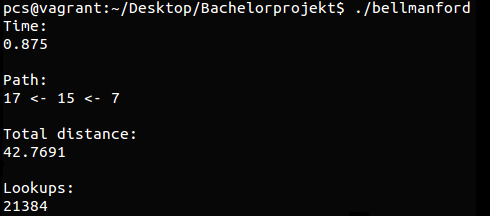
\includegraphics[scale=0.8]{Pictures/bellmanford-output.png}
\caption[]{Output from Bellman Ford implementation.}
\end{figure}

\begin{figure}[H]
\centering
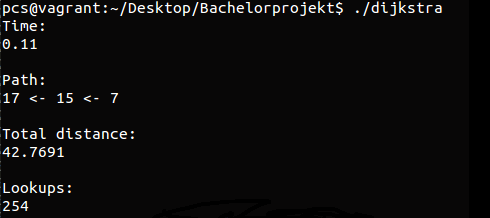
\includegraphics[scale=0.8]{Pictures/dijkstra-output.png}
\caption[]{Output from Dijkstra's algorithm implementation.}
\end{figure}

\begin{figure}[H]
\centering
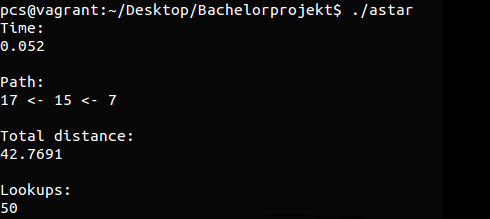
\includegraphics[scale=0.8]{Pictures/a-star-output.png}
\caption[]{Output from A* search implementation.}
\end{figure}

\end{document}